\documentclass{article}


% if you need to pass options to natbib, use, e.g.:
%     \PassOptionsToPackage{numbers, compress}{natbib}
% before loading neurips_2022


% ready for submission
% \usepackage{neurips_2022}


% to compile a preprint version, e.g., for submission to arXiv, add add the
% [preprint] option:
%     \usepackage[preprint]{neurips_2022}


% to compile a camera-ready version, add the [final] option, e.g.:
    \usepackage[final]{neurips_2022}


% to avoid loading the natbib package, add option nonatbib:
%    \usepackage[nonatbib]{neurips_2022}


\usepackage[utf8]{inputenc} % allow utf-8 input
\usepackage[T1]{fontenc}    % use 8-bit T1 fonts
\usepackage{hyperref}       % hyperlinks
\usepackage{url}            % simple URL typesetting
\usepackage{booktabs}       % professional-quality tables
\usepackage{amsfonts}       % blackboard math symbols
\usepackage{nicefrac}       % compact symbols for 1/2, etc.
\usepackage{microtype}      % microtypography
\usepackage{xcolor}         % colors


% -- 
\usepackage{enumitem}
% --- for professional tables
\usepackage{booktabs}  
% --- for figures
\usepackage{graphicx}
\usepackage{caption}
\usepackage{subcaption}
\usepackage{wrapfig}
% --- for formula
\usepackage{amssymb}
\usepackage{amsmath}
\DeclareMathOperator*{\argmax}{arg\,max}
\DeclareMathOperator*{\argmin}{arg\,min}
% --- for table and figure side by side
% \usepackage{floatrow}
\usepackage{makecell}
% Table float box with bottom caption, box width adjusted to content
% \newfloatcommand{capbtabbox}{table}[][\FBwidth]
% ----

\usepackage{multirow}
\usepackage{placeins}
\usepackage[normalem]{ulem}

% --- theorems
\usepackage{bbm}
\usepackage{amsthm}

\newtheorem{definition}{Definition}[section]
\newtheorem{example}{Example}[section]
\newtheorem{theorem}{Theorem}[section]
% \newtheorem{corollary}{Corollary}[theorem]
\newtheorem{lemma}[theorem]{Lemma}
\newtheorem{corollary}{Corollary}[section]
\newtheorem{proposition}{Proposition}[section]
% \newtheorem{remark}{Remark}[theorem]
% \newtheorem*{remark}{Remark}
\newtheorem{remark}{Remark}[section]
\newtheorem{assumption}{Assumption}[section]

% --- commands
\newcommand{\chengyu}[1]{{\color{blue}{\emph{CD: #1}}}}
% \newcommand{\chengyu}[1]{}
\newcommand{\todo}[1]{{\color{blue}{\textbf{TODO: #1}}}}
\newcommand{\jingbo}[1]{{\color{blue}{\textbf{Jingbo:} #1}}}
\newcommand{\lucas}[1]{{\color{red}{\textbf{lucas:} #1}}}
\newcommand{\lucasedit}[1]{{\color{gray}{#1}}}
\newcommand{\smallsection}[1]{\textbf{#1.~~~~}}
\newcommand{\note}[1]{{\color{red}{#1}}}

\newcommand{\noise}[1]{implicit label noise\xspace}
\newcommand{\Noise}[1]{Implicit label noise\xspace}

\newcommand{\specialcell}[2][c]{%
  \begin{tabular}[#1]{@{}c@{}}#2\end{tabular}}
  
  
% \title{Double Descent in Adversarial Training: An Implicit Label Noise Perspective}

% \title{Understanding Implicit Label Noise in Adversarial Training for Robust Deep Learning}
% \title{Label Noise Exists Implicitly in Adversarial Training}
% \title{Robust Overfitting May be Explained By the Label Noise in Adversarial Training}
% \title{Label Noise in Adversarial Training: A Novel Perspective to Explain and Alleviate Robust Overfitting}
\title{Label Noise in Adversarial Training: A Novel Perspective to Study Robust Overfitting}
% \title{Chart and harness the label noise in adversarial training}
% title based on 
% `Feature Purification: How Adversarial Training Performs Robust Deep Learning` Allen zhu.
% `UNDERSTANDING INTRINSIC ROBUSTNESS USING LABEL UNCERTAINTY`



% The \author macro works with any number of authors. There are two commands
% used to separate the names and addresses of multiple authors: \And and \AND.
%
% Using \And between authors leaves it to LaTeX to determine where to break the
% lines. Using \AND forces a line break at that point. So, if LaTeX puts 3 of 4
% authors names on the first line, and the last on the second line, try using
% \AND instead of \And before the third author name.


\author{%
Chengyu Dong \\
University of California, San Diego\\
\texttt{cdong@eng.ucsd.edu}\\
\And
Liyuan Liu\\
Microsoft Research\\
\texttt{lucliu@microsoft.com}\\
\And
Jingbo Shang\\
University of California, San Diego\\
\texttt{jshang@eng.ucsd.edu}\\
}


\begin{document}


\maketitle


\begin{abstract}

% \chengyu{Label noise exists -> explains overfitting -> double descent as a verification -> method to mitigate label noise}


% In adversarial training, inheriting labels for adversarial examples from their clean counterparts has been a common practice for years.
% In this paper, we argue that this common practice in fact leads to a mismatch between true label distribution and assigned label distribution, and therefore, introduces label noise to adversarial training implicitly. 
We show that label noise exists in adversarial training. 
Such label noise is due to the mismatch between the true label distribution of adversarial examples and the label inherited from clean examples 
% \jingbo{assigned label is not defined. I prefer the common practice way to describe this.} 
 -- the true label distribution is distorted by the adversarial perturbation, but is neglected by the common practice that inherits labels from clean examples. 
Recognizing label noise sheds insights on the prevalence of robust overfitting in adversarial training, and explains its intriguing dependence on perturbation radius and data quality. 
Also, our label noise perspective aligns well with our observations of the epoch-wise double descent in adversarial training. 
Guided by our analyses, we proposed a method to automatically calibrate the label to address the label noise and robust overfitting. 
Our method achieves consistent performance improvements across various models and datasets without introducing  new hyper-parameters or additional tuning.


% Here, we study the label noise issue for adversarial training. 
% We show that after adding adversarial perturbations to the original input, it is inevitable to shift the underlying label distribution.
% Correspondingly, it \jingbo{what is this ``it''? please try to make it more clear.} introduces label noise by inheriting labels from their clean counterparts for adversarial examples. 
% To examine the impact of label noise on adversarial training, we conduct empirical analyses on a label noise byproduct ( i.e., epoch-wise double descent) and observe a clear correlation between the level \jingbo{``the level'' reads a bit odd to me. degree? significance? idk.. and I think this part is not mentioned in intro now.} of epoch-wise double descent and the level of label noise. 
% Our observations verify our intuitions \jingbo{what are our intuitions? I would prefer to say it explicitly ``label noise exists in adversarial training''} and also shed insights on the the prevalence of robust overfitting in adversarial training. 
% Guided by our analyses, we proposed a method to automatically calibrate the label supervision to address the label noise and robust overfitting. 
% Our method achieves consistent performance improvements across various models and datasets without introducing  new hyper-parameters or additional tuning.


% Here, we study the a long-overlooked issue for adversarial training, i.e., implicit label noise. 
% We show that, adding adversarial perturbations to the original input image would cause the output  
% It is known that overfitting is more prominent in  adversarially robust deep learning than standard learning.
% In this paper, we extend the classic notion of label noise (label flipped for some instances) to implicit label noise (mismatch between true label distribution and assigned label distribution). 
% Under the perspective of implicit label noise, the prevalence of overfitting in adversarial training is properly aligned with the effect of label noise in standard learning in promoting variance. \jingbo{the last two ``in''s make me feel odd here.}
% We confirm that robust overfitting\jingbo{robust fitting is not mentioned before. We'd better to stick with the same term here.} can be viewed as a special case of epoch-wise double descent. 
% To mitigate implicit label noise in adversarial training, We show that model probability can approximate the true label distribution, in line with the existing practice in tackling robust overfitting. Finally, we show that it is possible to further boost the existing practice with temperature scaling and interpolation and validate its effectiveness by extensive experiments on benchmark datasets.



% In this paper, 
% we present the double descent phenomena in adversarial training and propose a novel perspective to understand it. 
% Specifically, 
% In this paper, we analyze robust overfitting from an epoch-wise double descent, i.e., we observe that the robust test error will start to decrease again after training the model for a considerable number of epochs.
% Inspired by our observations, 
% % we further tailored existing analyses and theory to better understand robust overfitting and the epoch-wise double descent. 
% we further advance the analyses of double descent to understand robust overfitting better. 
% \sout{In standard training, double descent has been shown to be a result of label flipping noise.}
% However, this reasoning is not applicable in our setting, since adversarial perturbations are believed not to change the label. 
% Going beyond label flipping noise, we propose to measure the mismatch between the assigned and (unknown) true label distributions, denoted as \emph{implicit label noise}.
% We show that the traditional labeling of adversarial examples inherited from their clean counterparts will lead to implicit label noise.
% % , but not label flipping noise.
% Towards better labeling, we show that predicted distribution from a classifier, after scaling and interpolation, can provably reduce the implicit label noise under mild assumptions.
% In light of our analyses, we tailored the training objective accordingly to effectively mitigate the double descent and verified its effectiveness on three benchmark datasets.



\end{abstract}


\section{Introduction}


% \chengyu{emphasize the focus of this work is to find out how does adversarial perturbation creates label noise, rather than to understand how label noise cause double descent}

% \chengyu{Introduce classic notion of label noise, new notion of label noise, then extend robust overfitting to double descent and join with effect of label noise in standard learning under this label noise perspective.}


Adversarial training~\citep{Goodfellow2015ExplainingAH, Huang2015LearningWA, Kurakin2017AdversarialML, Madry2018TowardsDL} is known as one of the most effective ways~\citep{Athalye2018ObfuscatedGG, Uesato2018AdversarialRA} to enhance the adversarial robustness of deep neural networks~\citep{Szegedy2014IntriguingPO, Goodfellow2015ExplainingAH}. 
It augments training data with adversarial perturbations to prepare the model for adversarial attacks. 
% can be viewed as a data augmentation technique that minimizes the empirical risk on an augmented set composed of adversarial training examples. 
Despite various efforts to generate more effective adversarial training examples~\citep{Ding2020MaxMarginA, Zhang2020AttacksWD},
% for adversarial training, 
the labels assigned to them attracts little attention. 
% In the common practice of adversarial training, 
As the common practice, the assigned labels of adversarial training examples are simply inherited from their clean counterparts. 

% In this paper, we argue that the existing labeling practice of the adversarial training examples may introduce label noise implicitly.
% It is known that adversarial perturbation can distort the data semantics~\citep{Tsipras2019RobustnessMB, Ilyas2019AdversarialEA}.
% \jingbo{since we are not going to say it's implicit label noise, shall we remove ``implicitly'' here?}
In this paper, we argue that the existing labeling practice of the adversarial training examples introduces label noise implicitly, since adversarial perturbation can distort the data semantics~\citep{Tsipras2019RobustnessMB, Ilyas2019AdversarialEA}.
% A small perturbation radius employed in adversarial training ensures that such semantic distortion is not significant enough to cause noisy labels. 
For example, as illustrated in Figure~\ref{fig:illustration}, even with a slight distortion of the data semantics (e.g., more ambiguous), the label distribution of the adversarially perturbed data may not match the label distribution of the clean counterparts.
Such distribution shift is neglected when assigning labels to adversarial examples, which are directly copied from the clean counterparts.
% From a statistical view of the annotation process, we define label noise as the empirical measure of label errors in a dataset. 
We observe that distribution mismatch caused by adversarial perturbation along with improper labeling practice will cause \emph{label noise
% \footnote{We define label noise as the empirical measure of label errors in a dataset.} 
in adversarial training}.


% \vspace{-4.0ex}
\begin{figure}[tp]
  \centering
  \includegraphics[width=1.00\textwidth]{figures/implicitLabelNoise.pdf}
%   \includegraphics[width=1.00\textwidth]{nips2022/figures/examples-low-quality-1.pdf}
  \vspace{-1ex}
  \caption{Illustration of the origin of label noise in adversarial training. 
  The adversarial perturbation causes a mismatch between the true label distributions of clean inputs $x$ and their adversarial examples $x'$. Such a distribution mismatch is however neglected by the labels assigned to adversarial examples in the common practice of adversarial training, resulting in label noise implicitly.
  % The traditional adversarial label introduces the implicit label noise by inducing a distribution mismatch between the assigned label distribution and true label distribution of the adversarial example. 
%   Using rectified model probabilities as assigned labels of adversarial examples can provably reduce this distribution mismatch.
%   \chengyu{Change pictures (needs to use 8/255 instead of 16/255, we don't want people to argue that this is exactly label noise), shrink, merge with Figure 1?}
  }
 \vspace{-2ex}
\label{fig:illustration}
\end{figure}

% Our label noise perspective brings a better understanding on robust overfitting, a prominent phenomenon in adversarial training~\citep{Rice2020OverfittingIA}.
It is a mysterious and prominent phenomenon that the robust test error would start to increase after conducting adversarial training for a certain number of epochs~\citep{Rice2020OverfittingIA}, and our label noise perspective provides an adequate explanation for this phenomenon. 
% A classic bias-variance view of model generalization suggests that overfitting can result from increased model complexity, while training longer can be viewed as one way to increase model complexity~\citep{Rice2020OverfittingIA}. Compared to standard training, label noise that implicitly exists in adversarial training can increase the model variance~\citep{Yang2020RethinkingBT} and thus make the overfitting much more evident.
Specifically, from a classic bias-variance view of model generalization, label noise that implicitly exists in adversarial training can increase the model variance~\citep{Yang2020RethinkingBT} and thus make the overfitting much more evident compared to standard training.
Further analyses of label noise in adversarial training also explain the intriguing dependence of robust overfitting on the perturbation radius~\citep{Dong2021ExploringMI} and data quality~\citep{Dong2021DataPF} presented in the literature. 


% \begin{figure} % {r}{0.9\linewidth} % [!ht]
\begin{wrapfigure}{r}{6cm} % [!ht]
  % \vspace{-4mm}
  \centering
  \includegraphics[width=1.0\linewidth]{figures/intro.pdf}
  \caption{Robust overfitting can be viewed as an early part of the epoch-wise double descent. 
  We employ PGD training~\citep{Madry2018TowardsDL} on CIFAR-10~\citep{Krizhevsky2009LearningML} with Wide ResNet (WRN)~\citep{Zagoruyko2016WideRN} and a fixed learning rate. 
%   We employ PGD training on CIFAR-10 with Wide ResNet (WRN) and a fixed learning rate. 
  WRN-$28$-$k$ refers to WRN with depth $28$ and widen factor $k$.
  }
\label{fig:intro}
\vspace{-3mm}
% \end{figure}
\end{wrapfigure}


% \jingbo{I wish to put the Figure 2 next to this paragraph. }
Providing the label noise in adversarial training, one can further expect the existence of double descent based on the modern generalization theory of deep neural networks.
% , which have never been reported in adversarial training. 
% Furthermore, modern generalization theory of deep neural networks has been shown to go beyond the classic bias-variance trade-off. 
\emph{Epoch-wise double descent} refers to the phenomenon that the test error will first decrease and then increase as predicted by the classic bias-variance trade-off, but it will decrease again as the training continues. Such phenomenon is only reported in standard training of deep neural networks, often requiring significant label noise in the training set~\citep{Nakkiran2020DeepDD}.
% When increasing model complexity by training longer, the resulting double descent is known as the epoch-wise double descent. 
% Joining the standard training, we show that implicit label noise also shares a similar effect in adversarial training. 
As the label noise intrinsically exists in adversarial training, such epoch-wise double descent phenomenon also emerges when the training goes longer.
% However, as robust overfitting is induced by the label noise implicitly exists in adversarial training, it should join such double descent phenomenon as the training goes longer. 
Indeed, as shown in Figure~\ref{fig:intro}, for a relatively large model such as WRN-28-5, on top of the existing robust overfitting phenomenon, the robust test error will eventually decrease again \emph{after $1,000$ epochs}. Following \cite{Nakkiran2020DeepDD}, we further experiment different model sizes. One can find that a medium-sized model will follow a classic U-curve, which means only overfitting is observed; and the robust test error for a small model will monotonically decrease. These are well aligned with the observations in standard training regime.
% This verifies our understanding of label noise in adversarial training.
This again consolidates our understanding of label noise in adversarial training.
% \jingbo{there are two more curves in the figure. we should also talk about them?}



In light of our analyses, we design a theoretically-grounded method to mitigate the label noise in adversarial training automatically.
The key idea is to resort to an alternative labeling of the adversarial examples. 
We show that the predictive label distribution of an adversarially trained probabilistic classifier can approximate the true label distribution with high probability. Thus it can be utilized as a better labeling of the adversarial examples and provably reduce the label noise. We also show that with proper temperature scaling and interpolation, such predictive label distribution can further reduce the label noise.
% We show that the predictive label distribution of a probabilistic classifier adversarially trained as usual, but after being properly scaled and interpolated, can be utilized as a better labeling of the adversarial examples and provably reduce the implicit label noise. 
This echoes the recent empirical practice of incorporating knowledge distillation~\citep{Hinton2015DistillingTK} into adversarial training~\citep{chen2021robust}. 
While previous works heuristically select fixed scaling and interpolation parameters for knowledge distillation, we show that it is possible to fully unleash the potential of knowledge distillation by automatically determining the set of parameters that maximally reduces the label noise, with a strategy similar to confidence calibration~\citep{Guo2017OnCO}. 
Such strategy can further mitigate robust overfitting to a minimal amount without additional human tuning effort.
Extensive experiments on different datasets, training methods, neural architectures and robustness evaluation metrics verify the effectiveness of our method.



In summary, our findings and contributions are: 1) we show that the labeling of adversarial examples in adversarial training practice introduces label noise implicitly; 2) we show that robust overfitting can be adequately explained by such label noise, and it is the early part of an epoch-wise double descent; 3) 2e show an alternative labeling of the adversarial examples can be established to provably reduce the label noise and mitigate the robust overfitting.  

% \begin{itemize}[leftmargin=2em, topsep=0pt,itemsep=-0.5ex,partopsep=1ex,parsep=1ex]
%     \item We show that the labeling of adversarial examples in adversarial training practice introduces label noise implicitly.
%     \item We show that robust overfitting can be adequately explained by such label noise, and it is the early part of an epoch-wise double descent.
%     % \item We show that robust overfitting shall be viewed as the early part of an epoch-wise double descent, extending the common belief in adversarial training. Robust overfitting can thus be incorporated into the existing understanding of double descent.
%     % \item We show that double descent in adversarial training may originate from the implicit label noise introduced by improper \jingbo{maybe say imperfect? we argued that the common practice is correct if it has to be one-hot labels} labeling of adversarial examples in adversarial training practice.
%     \item We show an alternative labeling of the adversarial examples can be established to provably reduce the label noise and mitigate the robust overfitting.  
%     % \jingbo{maybe mention minimal human effort or something similar? }
% \end{itemize}

% The remainder of this paper is organized as follows.
% In Section~\ref{sect:related}, we briefly review the existing works on robust overfitting.
% In Section~\ref{sect:reason}, we explore the origin of label noise in adversarial training and analyze its dependence.
% In Section~\ref{sect:mitigate-double-descent}, we propose to mitigate robust overfitting by alternative labeling.
% Section~\ref{sect:experiment} demonstrates the effectiveness of our method on realistic datasets. 
% Conclusions and further implications are discussed in Section~\ref{sect:conclusion}.









% Adversarial training is a popular technique for robust deep learning...

% Adversariral training can be viewed as training on an augmented dataset~\cite{Tsipras2019RobustnessMB}, where the assigned labels are directly copied from the assigned labels of clean inputs.
% We argue that such common practice introduce label noise implicitly. By a distribution mismatch, although no conventional definition of label noise is observed.

% Explains robust overfitting.

% Double descent confirms this label noise view. 

% Mitigate double descent.





% \chengyu{Here goes the old version.}

% In adversarial training, a typical phenomenon is that after a certain training epoch, the robust test error will start to increase constantly with further training, despite the robust training error continues to decrease~\citep{Rice2020OverfittingIA}. 
% \sout{This phenomenon, known as \emph{robust overfitting}, is believed to be separated from \emph{double descent}~\citep{Belkin2019ReconcilingMM} in the literature~\citep{Rice2020OverfittingIA}.} 

% % In contrast to the common belief that deep networks hardly overfit in standard training~\citep{Zhang2017UnderstandingDL, Neyshabur2017ExploringGI}, overfitting has been shown to be a dominant phenomenon in adversarially robust training~\citep{Rice2020OverfittingIA}.
% % After a certain point during training, the robust test error will start to increase constantly with further training, despite the robust training error continues to decrease. 
% % This phenomenon, known as ``\emph{robust overfitting}'', is believed to be separated from \emph{double descent}~\citep{Belkin2019ReconcilingMM} in previous works~\citep{Rice2020OverfittingIA}. 



% Here, we find that robust overfitting\jingbo{Robust overfitting not defined in intro} shall be viewed as the early part of an epoch-wise double descent~\citep{Nakkiran2020DeepDD}.
% % after conducting adversarial training for sufficiently many epochs. 
% As shown in Figure~\ref{fig:intro}, for relatively large models \jingbo{I think you want to refer to the medium size one in the figure? if so name it.}, the robust test error increases only transiently and will eventually decrease again after a considerable number of training epochs. 
% Modulating the model architecture size can shifting the epoch-wise double descent curve such that either the overfitting curve is shown \jingbo{probably refer to the model name here and also in the other part of ``or'' clause.}, or the entire double descent curve is revealed within the same number of training epochs.
% % as shown in Figure~\ref{fig:intro}. 
% % Therefore, Robust overfitting should be unified with double descent and 
% % Our analyses thus manage to unifying the two seemingly separately phenomena. % robust overfitting and double descent.
% In Appendix~\ref{sect:double-descent-reconcile}, we verify our observation across various training settings such as different sample sizes, optimizers, learning rate schedulers, and neural architectures.
% Therefore, robust overfitting will not go beyond modern generalization theory as an exception and should be incorporated into the existing understanding of \jingbo{I think some reviewers mentioned the issue of mixing model-wise and epoch-wise double descent. Probably we want to make it very clear this time.} double descent.
% % adequately explained by the origin of double descent such as label noise.
% % In Appendix~\ref{sect:double-descent-reconcile}, we observe consistent and similar patterns across various training settings (e.g., different sample sizes, optimizers, learning rate schedulers, and neural architectures)

% % , which further verifies our intuition 
% % that robust overfitting shall be viewed as the early part of an epoch-wise double descent (see Appendix~\ref{sect:double-descent-reconcile}).
% % \jingbo{the last sentence is a little repeated?}
% % \lucas{how about verifies the connection between the robust overfitting, and the double descent?}
% % on the connection between the robust overfitting and the double descent (See ). 

% % \chengyu{Previous works suggest that those hard examples in adversarial training might be label noise after adversarial perturbation (`Explore memorization`). However, we carefully inspect the hardest examples and find that they are at most more ambiguous. Nevertheless, we show that label noise can implicitly exist in adversarial training even though all assigned labels are correct. ...} 
% % \chengyu{Discuss that ``hard examples might be label noise'' mentioned in `exploring memorization...`, just show the hardest examples with $8/255$ perturbation and are at most ambiguous.} 


% % In our study, we aim to better understand the 
% % Motivated by our observations, we aim to adopt the double descent perspective to better understand the robust overfitting.  
% % Inspired by this observation, we further analyze the epoch-wise double descent to better understand the robust overfitting.
% % Inspired by the above observation
% We further explore the origin of the double descent in adversarial training to better understand robust overfitting.
% % propose to understand the double descent in adversarial training from an \emph{implicit label noise} perspective.
% In standard training, 
% % the double descent is shown to be related to the label noise~\citep{}. Specifically, 
% to observe the double descent for modern neural architectures it is often necessary to manually inject label noise~\citep{Nakkiran2020DeepDD, Yang2020RethinkingBT}.
% However, adversarial perturbations are believed to not change the underlying labels, \jingbo{shall we make it clear that it's the one-hot label?} % or introduce label noise.
% % We further empirically confirm that adversarial perturbation is unlikely to change the argmax label. \jingbo{this argmax label might be confusing.}
% which is further confirmed empirically from our manual inspection. 
% Therefore, label noise \jingbo{since we will implicit label noise later, we should define it clearly what is label noise or at least use something like (e.g., label flipped) to explain it along with some citation} should not explicitly exist in adversarial training.
% % Therefore, the popular label flipping noise explanation is not applicable here. 
% % We note that the common practice of directly copying labels from clean examples to their adversarial counterparts may introduce label noise, which is essential to produce double descent in model neural architectures~\citep{Nakkiran2020DeepDD, Yang2020RethinkingBT}.
% % However, based on our empirical checks and literature \jingbo{cite the work you mentioned later}, adversarial perturbation is unlikely to change the argmax label; therefore, the popular label flipping noise explanation \jingbo{maybe a citation here} is not applicable here. 
% On the other hand, it is reasonable to believe that adversarial perturbation distorts the label distribution since the data examples do become more ambiguous after perturbation. 
% Such perturbation thus induces a mismatch between the assigned label distribution \jingbo{What is assigned label distribution? not clear here.} and (unknown) true label distribution, which leads to \emph{implicit label noise}.
% % Thus, we focus on the \emph{implicit label noise} which measures the mismatch between the assigned label distribution and (unknown) true label distribution. 
% We show such implicit label noise can be interpreted as a specific type of label noise and can have a great impact in adversarial training, which thus provides a new perspective to understand the double descent in adversarial training. Indeed, extensive analyses of implicit label noise can explain the intriguing dependency of robust overfitting on perturbation size~\citep{Dong2021ExploringMI} and data quality~\citep{Dong2021DataPF}.
% % \lucas{maybe we start from the contradict between the label flipping noise, and the adversarial training practice?}

% % Our implicit label noise perspective can further inspire novel adversarial algorithms to mitigate the double descent.
% Guided by our analyses, we design a theoretically-grounded method to mitigate the robust overfitting.
% % A natural idea is to resort to an alternative labeling of the adversarial examples. 
% The key idea is to resort to an alternative labeling of the adversarial examples. 
% We show that the predictive label distribution of a probabilistic classifier adversarially trained as usual, but after being properly scaled and interpolated, can be utilized as a better labeling of the adversarial examples and provably reduce the implicit label noise. 
% This echoes the recent empirical practice of incorporating knowledge distillation~\citep{Hinton2015DistillingTK} into adversarial training~\citep{chen2021robust}. 
% While previous works heuristically select fixed scaling and interpolation parameters for knowledge distillation, we show that it is possible to fully unleash the potential of knowledge distillation by automatically determining the set of parameters that maximally reduces the implicit label noise, with a strategy similar to confidence calibration~\citep{Guo2017OnCO}. 
% Such strategy can further mitigate robust overfitting to a minimal amount without additional human tuning effort.
% % without additional tuning.
% % \jingbo{is this ``minimal amount'' supported by any of our exps? otherwise, let's remove this suffix.}
% % Extensive experiments on different datasets, training methods, neural architectures and robustness evaluation metrics demonstrate our approach can effectively mitigate robust overfitting.
% Extensive experiments on different datasets, training methods, neural architectures and robustness evaluation metrics verify the effectiveness of our method.

% In summary, our findings and contributions are as follows.
% \begin{itemize}[leftmargin=2em, topsep=0pt,itemsep=-0.5ex,partopsep=1ex,parsep=1ex]
%     % \item We challenge the common belief that the robust overfitting and double descent are separate phenomena and show that robust overfitting is an early part of epoch-wise double descent. % the in adversarial training with the  
%     \item We show that robust overfitting shall be viewed as the early part of an epoch-wise double descent, extending the common belief in adversarial training. Robust overfitting can thus be incorporated into the existing understanding of double descent.
%     \item We show that double descent in adversarial training may originate from the implicit label noise introduced by improper \jingbo{maybe say imperfect? we argued that the common practice is correct if it has to be one-hot labels} labeling of adversarial examples in adversarial training practice.
%     \item We show an alternative labeling of the adversarial examples can be established to provably reduce the implicit label noise and mitigate the robust overfitting. 
% \end{itemize}

% % \jingbo{Since our submission doesn't follow the conventional related work--method--exp--conclusion flow, I think it's a good idea to put a paragraph here to explain how the write-up is organized. }

% The remainder of this paper is organized as follows.
% In Section~\ref{sect:related}, we briefly review the existing works that explore robust overfitting and double descent.
% In Section~\ref{sect:reason}, we theoretically explore the origin of double descent in adversarial training from an implicit label noise perspective.
% In Section~\ref{sect:mitigate-double-descent}, we propose to mitigate the double descent in adversarial training by alternative labeling based on our understanding. Section~\ref{sect:experiment} demonstrates the effectiveness of our method on realistic datasets. 
% Conclusions and further implications are discussed in Section~\ref{sect:conclusion}.

version https://git-lfs.github.com/spec/v1
oid sha256:f56b76354e3226b92438446f15b0d9b8c07c1437aed620bcb3a8be06906e82ae
size 11925

version https://git-lfs.github.com/spec/v1
oid sha256:7e1d914ab759c5b6dbfbf25ab730016ecf474362d6da8410b5525ba0d9b620c1
size 13827

% \section{Double Descent from an Implicit Label Noise Perspective}
% \section{Adversarial perturbation can cause label noise implicitly}
% \section{Explore Label Noise in Adversarial Training}
% \label{sect:reason}

% \chengyu{Make sure we show the point that adversarial training only \emph{magnifies} the label noise and thus makes the robust overfitting more evident.}

% \chengyu{Avoid mention double descent to the best}

% \chengyu{maybe also no need to define ``implicit label noise''. Then people will not require us to demonstrate such a new type of label noise in the reality.}

% In this section, we present a novel perspective to understand the double descent in adversarial training. The implicit label noise is originated from the improper labeling of the adversarial examples and can induce double descent in adversarial training.

% In this section, we first show that traditional adversarial perturbation does not cause label noise directly. We then argue that adversarial perturbation cause label noise implicitly, but significantly.

% To understand intriguing behaviors of adversarial training such as robust overfitting we focus on its training set. We first show that label noise does not explicitly exist in the adversarially augmented training set. We then argue that label noise will implicitly exist in the adversarially augmented training set due to the distribution mismatch and improper label construction in the common practice.


 




% % ----------------------------------------------
% ----------------------------------------------
% \subsection{Traditional adversarial label \textbf{does not introduce label flipping noise}}
% \subsection{Traditional adversarial label does not introduce label noise directly}
\subsection{Label noise does not explicitly exist in the adversarially augmented training set}
\label{sect:label-flipping-noise}

\chengyu{Remove this section?}
% \sout{In standard learning, it is often necessary to manually inject label noise to make the double descent evident for modern neural architectures~\citep{Nakkiran2020DeepDD, Yang2020RethinkingBT}.}

% Since label noise is often essential to explain double descent in standard learning for modern neural architectures~\citep{Nakkiran2020DeepDD, Yang2020RethinkingBT},
% We wish to check if the traditional adversarial label produces any label flipping noise, a typical type of label noise, namely if $\tilde{y}_\delta \ne y^*_\delta$ for any adversarial example $x_\delta$.
% \chengyu{It is still possible there is a tiny fraction of label noise. But won't make a big difference.}
% the assigned label of the adversarial example is different from its true label.
% This is equivalent to checking if $ y^* \ne y_\delta^* $, since $\tilde{y}_\delta = y$ by the definition of the traditional adversarial label (Definition~\ref{remark:common-practice}) and $y = y^*$ by the property of our clean dataset (Assumption~\ref{assumption:clean-dataset}). Note that $y^* \ne y_\delta^*$ means the semantics of the adversarial example is distorted significantly such that its argmax label is now different from the argmax label of its clean counterpart. % , which is possible under adversarial perturbation.


    % The common practice in adversarial training assumes that an adversarial example shares the same true label with its clean counterpart, i.e., $\hat{y}_{\delta} \leftarrow \hat{y}$.
    % Since we have to pick one label for each instance and we have assumed $p(\hat{y} | x) = p(y | x)$, this assumption can be formally viewed as ``$\argmax_j ~p(y_{\delta}=j|x + \delta) = \argmax_j ~p(y=j|x)$''. 
    % Here, we show that this assumption does not introduce label flipping noise, which is often necessary to produce double descent in modern neural architectures in standard classifier training.


% \begin{figure*}[!ht]
% \centering
% % \begin{subfigure}{1.0\textwidth}
%   \centering
%   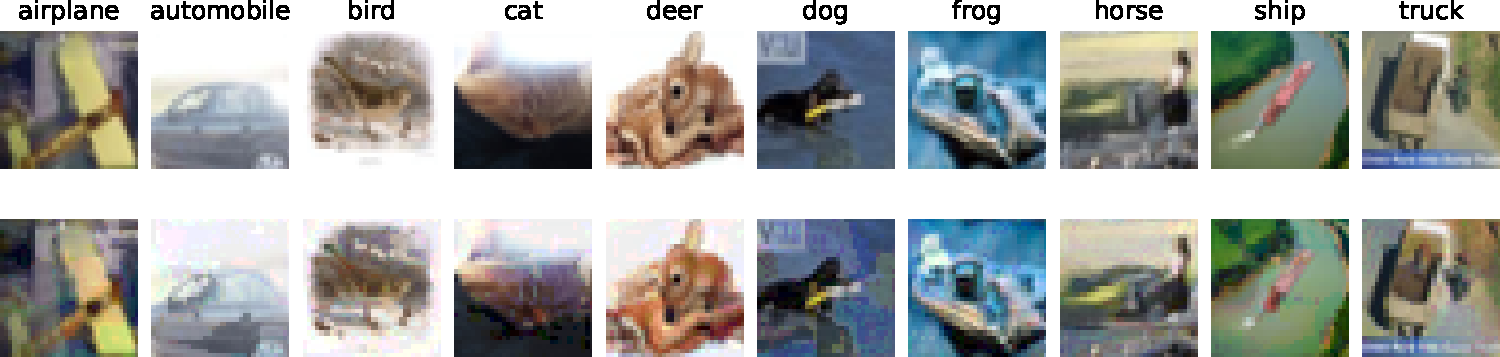
\includegraphics[width=0.95\linewidth]{figures/examples-low-quality.pdf}
%   % \caption{Examples with the lowest quality and their corresponding adversarial examples.}
%   % \label{fig:problematic-examples-orig}
% % \end{subfigure}
% % \begin{subfigure}{1.0\textwidth}
% %   \centering
% %   \includegraphics[width=0.95\linewidth]{figures/examples-high-quality.pdf}
% %   \caption{Examples with the highest quality and their corresponding adversarial examples.}
% %   \label{fig:problematic-examples-ad}
% % \end{subfigure}
%   \caption{Examples with the lowest and highest quality identified in the training set of CIFAR-10. In each subfigure, the top row shows the original image and the bottom row shows the image after the adversarial perturbation (PGD-10 with perturbation radius $8/255$). For each image, the true label is annotated on the top.}
%   % , and the predicted label is annotated on the bottom.}
% \label{fig:examples}
% \end{figure*}



We check if the adversarially augmented training set constructed from the benchmark dataset contains any noisy labels, namely the assigned labels that are different from their corresponding true labels.
    % We first visually check the adversarial examples created by the inner maximization in adversarial training. 
    We are specifically interested in those inputs with the lowest data quality as they are mostly likely to become label noise after perturbation.
    We estimate data quality based on model ensemble (see Appendix~\ref{sect:data-quality-estimation}).
    One can find that the adversarial examples of those low-quality inputs still match their original labels, albeit being slightly more ambiguous (see Figure~\ref{fig:illustration} and \todo{more samples in Appendix.}). 
    
    Evidence can also be found by charting the geometrical structure of the benchmark dataset.
    % \citet{Yang2020ACL} study the distance between examples in the input space. 
    In CIFAR-10 training set, \citet{Yang2020ACL} found that the minimum distance between any two inputs with different labels is around $50/255$ in terms of $\ell_\infty$ norm. In contrast, the perturbation radius used in adversarial training is typically $8/255$, which is significantly smaller. Therefore, it is unlikely that adversarial perturbation will change the true labels of the training inputs.
    It is thus reasonable to argue that label noise does not explicitly exist in the adversarially augmented training set in abundance.
    % Subsequently it cannot adequately explain the double descent observed in adversarial training.

version https://git-lfs.github.com/spec/v1
oid sha256:9956ecf8f72f8cc864de3724da585c24c2cb6e97975537af55723da00e24101f
size 19514


% \subsection{Equivalence between implicit label noise and label flipping noise}
% \subsection{Influence of implicit label noise in adversarial training}
% \subsection{Influence of implicit label noise}
% \subsection{Implicit label noise is a specific type of label noise}
% \smallsection{Connection and difference between implicit label noise and conventional label noise}
\smallsection{Intuitive interpretation of label noise in adversarial training}
% \chengyu{If no section 4.1, can also remove this section}
% In this section, we connect the implicit label noise to a more familiar definition of label noise and show it can have a significant impact.
%     \begin{proposition}[Implicit label noise is equivalent to instance-dependent and class-dependent label noise]
%     \label{proposition:label-noise}
%     Let $p_e(j, x) = P(\tilde{Y}\ne j | Y = j, x)$ be a typical definition of label noise which depends on both the class $j$ and input $x$. Then implicit label noise is equivalent to
%     \begin{equation}
%       % p(Y\ne Y^* | x) = 1 - \sum_j p(Y= j | Y^* = j, x) p(Y^* = j|x),
%       P(\tilde{Y}\ne Y | x) = 1 - \sum_j (1 - p_e(j, x)) P(Y = j|x),
%     \end{equation}
%   % It can easily seen that if $p(Y\ne Y^* | x) > 0$, $p(Y\ne j | Y^* = j, x) > 0$ for some $j$.
%   \end{proposition}
%   \begin{proof}
%   See Appendix~\ref{sect:label-noise-more-proof}.
%   \end{proof}
We introduce a simple example to help understand the emergence of label noise in adversarial training.
% Towards an intuitive understanding of implicit label noise, we introduce a simple example to discuss the differences and connections between implicit label noise and convention label noise.
% We now try to quantify the implicit label noise given its connection with typical label noise.
% \chengyu{We now discuss a simplified example of implicit label noise, and discuss its connection and difference with conventional label noise.}
\begin{example}
% [Quantify the implicit label noise]
[Label noise due to a symmetric distribution shift]
\label{example:label-noise-influence}
% We would like to note that the adversarial training setting would amplify the impact of the implicit label noise, since it adds perturbations to every training sample. 
% In fact, Theorem 3.1 in our main paper, which lower-bounds the implicit label noise by the distance between the assigned label distribution and the true label distribution, provides a way to intuitively quantify the implicit label noise. 
Let $\mathcal{D}=\{(x_i, y_i)\}_{i\in[N]}$ be a clean labeled training subset where all inputs $x_i=x$ are identical and have a one-hot true label distribution, i.e., $P(Y|x) = \mathbf{1}_y$. %, and there is no label noise in $\mathcal{D}$, i.e. $y = \tilde{y}$. 

We now construct an adversarially augmented training subset $\mathcal{D'} = \{(x'_i, \tilde{y}'_i)\}_{i\in[N]}$, where $\tilde{y}' = y$ and $x'$ is generated based on adversarial perturbation that distorts the true label distribution symmetrically. Specifically,
$$
P(Y'= j' | x') =
\begin{cases} 
1 - \eta, & \text{if}~~j = y, \\
\eta/(K-1), & \text{otherwise}. \\
\end{cases}
$$
Then by Lemma~\ref{theorem:implicit-label-noise} 
% we have $P(\tilde{Y}' \ne Y' | x') \ge \eta$.
% we have $E_{j'} P_e(j', x') \ge \eta$.
we have $p_e (\mathcal{D}')\gtrsim \eta$.
% \ge % \left\| P(Y^*|x) -  P(Y^*_\delta|x_\delta).\right\|_{\text{TV}}
% which is equivalent to $p_e(j,x) = \sigma$ by Proposition~\ref{proposition:label-noise}. % , meaning $10\%$ label noise is injected in $\mathcal{S}$.
% which means the label noise injected in $\mathcal{S}_\delta$ is at least $10\%$  by Proposition~\ref{proposition:label-noise}.
% the total variation distance between these distributions is 0.1, which means the implicit label noise is at least 0.1. This is already equivalent to 10\% label noise based on the connection between implicit label noise and the (instance-wise) probabilistic definition of label flipping noise (see Remark 3.2 in our paper).
% \jingbo{what is this 10? I didn't quite get this.}
\end{example}
   
% \chengyu{Talk about observation distribution, noisy process and true distribution?}

One can find that there is indeed $\eta$ faction of noisy labels in $D'$. This is because if we sample the labels of $x'$ based on its true label distribution, we expect $1 - \eta$ faction of $x'$ are labeled as $y$, while $\eta$ fraction of $x'$ are labeled to be other classes. However, in $D'$, all $x'$ are assigned with label $y$ , which means $\eta$ fraction of $x'$ are labeled incorrectly. In realistic datasets we can consider inputs with similar features for such reasoning.

% \chengyu{Add a interpretation from population view?? I remember there is a case about dogs and cats in previous revision.}
% Conventionally speaking, label noise is perceived as the fraction of the noisy labels in the training set, i.e. the assigned labels that are different from their corresponding true labels. However, in the adversarially augmented training set no assigned label is noisy since $\tilde{y}' = y'$ 
% ~\footnote{Recall $\tilde{y}' = \argmax_j P(\tilde{Y'}=j|x')$ and $y' = \argmax_j P(Y'=j|x')$}
% for every augmented input $x'$. Yet, rather counter-intuitively, at least $\eta$ label noise exists in $\mathcal{D}'$, which is due to the fact that every input is now more likely to be mislabeled after adversarial perturbation.


% \chengyu{Difference from a process view. There is no noisy process defined, only the final assigned distribution after noisy process is known. But as long as the final distribution is different, suggests the annnotation must go through some unknown noisy process.}
% \chengyu{Why same argmax doesn't mean there is no label noise? Because label noise is always associated with a noisy random process. Because the change of the underlying true distribution should be reflected in the sampled labels, otherwise there must be some noisy process an annotator goes through.}

The above example also shows that label noise in adversarial training may be stronger than one's impression. Even a slight distortion of the true label distribution, e.g. $\eta=0.1$, will be equivalent to at least $10\%$ noisy label in the training set. This is because the true label distribution of every training input is distorted, resulting in significant noise in the population. 
% \sout{Such example also implies that even static adversarial perturbation~\footnote{namely the adversarial perturbation is added to the training set only once and the standard training is performed subsequently} can produce clear double descent as shown in Appendix~\ref{sect:exp-static}.} Therefore we believe implicit label noise can be an important source of label noise that makes double descent more evident in adversarial training.



    % An informal proof can be sketched from a frequentist's view and help the understanding of implicit label noise.
    % % One can interpret the implicit label noise in a frequentist's view.
    % Say there are $M$ identical copies of $x_\delta$ in the training set $\mathcal{D}_\delta$, with their true labels and traditional adversarial labels distributing according to $p(y^*_\delta | x_\delta)$ and $p(\tilde{y}_\delta| x_\delta)$, respectively.
    % % by Remark~\ref{remark:common-practice} and Assumption~\ref{assumption:clean-dataset}, respectively.
    % % The true label of $x_\delta$ is sampled based on $p(y_\delta |x + \delta)$, the assigned label is sampled based on $p(y|x)$. 
    % The number of copies that have the same true label and assigned label is $ M \sum_j \min \{p(\tilde{Y}_\delta=j|x_\delta), p(Y^*_\delta=j |x_\delta)\}$.
    % The fraction of label noise exists in $\mathcal{D}_\delta$ is thus $1 - \sum_j \min \{p(\tilde{Y}_\delta=j|x_\delta), p(Y^*_\delta=j|x_\delta)\} = \|p(\tilde{y}_\delta|x_\delta) - p(y^*_\delta|x_\delta) \|_{\text{TV}}$  by the definition of the total variation distance.
    


version https://git-lfs.github.com/spec/v1
oid sha256:bd53bfcdc9be7719f7641df9282fe65e2294c13aba7d9dc741aedcf6f9e5c09a
size 6797


\subsection{Adversarial perturbation generated by a realistic classifier}
\label{sect:reason-realistic}
We now consider a realistic case where the adversarial perturbation is generated by a probabilistic classifier $f_\theta$. 

% \begin{lemma}[Change of the predictive distribution after adversarial perturbation]
% Assume FGSM, cross-entropy loss.
% Assume $f_\theta(x)_y$ is $L$-locally Lipschitz. 
% \chengyu{copy from the proof of true probabilistic classifier Theorem 4.1 and Corollary 4.1}
% \begin{equation}
%     % \|P(Y|x) - P(Y'|x')\|_{\text{TV}} \ge
%         % \frac{\varepsilon}{2} (1 - q(x)) \frac{m}{L}  - \frac{\varepsilon^2}{4} M.
%     \|f_\theta(x') - f_\theta(x)\|_{\text{TV}} \ge
%         \frac{\varepsilon}{2} (1 - f_\theta(x)_y) \frac{m}{L}  - \frac{\varepsilon^2}{4} M.
% \end{equation}
% \end{lemma}

\smallsection{Approximation of the true label distribution}
% \chengyu{need to introduce some intuition here..}
We show that after sufficient adversarial training, the predictive label distribution of $f_\theta$ can approximate the true label distribution with high probability. 
% Therefore, an additional error term will be required to lower bound the label noise compared to the ideal case.
% We show that a probabilistic classifier trained on the conventional adversarially augmented training set can learn the true label distribution.
% Although we only have one-hot labels, but note that in the clean dataset one-hot label is an unbiased estimate of the true label distribution, namely $\mathbb{E}[\mathbf{1}_y] = P(Y|x)$.
% \chengyu{No, it is a biased-estimation... But it is close to true by Lipschitz}
% Thus given a collection of training inputs with the same true label distribution, the sample mean of their one-hot labels converges to the true label distribution.
% \chengyu{group and then relaxation}
\begin{lemma}% [Classifier by adversarial training learns the true label distribution]
\label{lemma:Learn-true-distribution}
% Assume the function generating the true label distribution $\mathbf{p}^*: \mathcal{X} \rightarrow \mathcal{Y}$ is $L^*$-locally Lipschitz continuous in a norm ball of radius $r$ around $x \in \mathcal{X}$.
% Select the loss function $\ell(\cdot, \cdot)$ to be a proper scoring rule.
% \chengyu{Only need to consider one particular adversarially augmented dataset here $D' = \{(x', \tilde{y})$, then any other points within metric ball will approximate true distribution with Lipschitz bound?}
Denote $\mathcal{S} = \{x: (x,y)\in \mathcal{D}\}$ as the collection of all training inputs.
Let $\rho\ge 1$ and $\mathcal{C}$ be an $\rho\varepsilon$-external covering of $\mathcal{S}$ with covering number $N_{\rho\varepsilon}$.
% Let $\{\mathcal{S}_i\}_{i\in [N_s]}$ be a disjoint partition of $\mathcal{S}$ induced by $\mathcal{C}$.
% Let $\mathcal{F}_{L, r}$ be a family of functions that are $L$-locally Lipschitz continuous in a norm ball of radius $r$ around $x \in \mathcal{C}^r$.  
Let $f_\theta$ be a probabilistic classifier that minimizes the adversarial empirical risk (\ref{eq:outer-minimization}).
% , namely
% This ensures all $x'$ in the norm ball is minimized, thus all $x'$ in the norm ball have true label distribution predicted.
% \begin{equation}
%     \label{eq:lip-minimization}
%     \theta = \argmin_\theta \frac{1}{|D|}\sum_{(x,y) \in D} \max_{x'\in \mathcal{B}_\varepsilon(x)}\ell (f_\theta(x'), y),
% \end{equation}
Assume $f_\theta$ is $L_\theta$-locally Lipschitz continuous in a norm ball of radius $\rho\varepsilon$ around $x \in \mathcal{C}$.
Let $\kappa \ge 1$ and $ \mathcal{\hat{S}}$ be a subset of $\mathcal{S}$ with cardinality at least $(1 - 1/\kappa + 1/(\kappa N_{\rho\varepsilon})) N$.
Let $\mathcal{N}_\varepsilon(\mathcal{\hat{S}})$ denote the neighborhood of the set $\mathcal{\hat{S}}$, i.e. $\mathcal{N}_\varepsilon(\mathcal{\hat{S}}) = \bigcup_{x\in\mathcal{\hat{S}}} \mathcal{B}_\varepsilon (x)$. 
Then for any $x \in \mathcal{N}_\varepsilon(\mathcal{\hat{S}})$, with probability at least $1-\delta$,
 
\begin{equation}
    \label{eq:main-theorem-bound}
    \|f_\theta(x) - P(Y|x)\|_{\text{TV}} \le \sqrt{\frac{\kappa N_{\rho\varepsilon} K}{2N}\log\frac{2}{\delta}}  + \left(\left(\frac{3}{2} - \frac{1}{K}\right) L_\theta + L\right) \rho \varepsilon,
\end{equation}
% where $\xi_K = \frac{1}{2}( 1 + K\|\mathbf{1}_{\circ} - K^{-1}\mathbf{1}\|_1)$.
% Here $\mathbf{1}_{\circ} \in \mathbb{R}^K$ denotes the one-hot vector where an arbitrary entry is $1$. 

% \chengyu{If it is anywhere robust, then it must be robust to manifold perturbation? But how large the perturbation is manifold perturbation that a model should be robust to? Is true model robust to manifold perturbation?}
% \chengyu{What's relation between $r$ and $\varepsilon$?}

% x' include x
% With probability $1-\delta'$, 
% $$
% |f_\theta(x') - f(x')| \le o(\delta')
% $$
\end{lemma}



% \chengyu{Talk about relation to the conventional robustness generalization bound (requires more stringent Lipschitz)}




\smallsection{Label noise in adversarial training with a realistic classifier}
% \chengyu{Or we prove that any perturbation that distort the output of a robust model is likely to at least partially distort the true label distribution?}
Adversarial perturbation generated by a realistic classifier $f_\theta$ will distort its predictive label distribution by gradient ascent. Subsequently, the true label distribution will also be distorted with high probability since the predictive label distribution of a realistic classifier $f_\theta$ can approximate the true label distribution. Specifically, by the triangle inequality we have
\begin{equation}
\|P(Y|x)  - P(Y'|x') \|_{\text{TV}} \ge \|f_\theta(x)  - f_\theta(x')\|_{\text{TV}} - (\|f_\theta(x) - P(Y|x)\|_{\text{TV}} + \|f_\theta(x') - P(Y'|x')\|_{\text{TV}}),
\end{equation}
where the last two terms are the approximation error of true label distribution on both clean and adversarial examples, which are guaranteed to be small. To conclude, we have the following result.
\begin{theorem}
\label{theo:realistic-classifier}
Instantiate the notations of Lemma~\ref{lemma:Learn-true-distribution}. For any $x \in \mathcal{N}_\varepsilon(\mathcal{\hat{S}})$, with probability at least $1 - 3\delta$, we have
\begin{equation}
    % \|P(\tilde{Y}'|x) - P(Y'|x)\|_{\text{TV}} \ge
    % \varepsilon \left[(1 - f_\theta(x)_y) \frac{m}{2L_\theta}- \rho\left(\left(\frac{3}{2} - \frac{1}{K}\right) L_\theta + L\right)\right]  - \varepsilon^2\frac{M}{4}  
    % %  \|f_\theta(x)  - f_\theta(x')\|_{\text{TV}}
    % - \sqrt{\frac{2\kappa N_s K}{N}\log\frac{2}{\delta}}
    p_e(\mathcal{D}') \ge
    \varepsilon \left[(1 - \mathbb{E}_x f_\theta(x)_y) \frac{\sigma_m}{2L_\theta}- 2\rho\left(\left(\frac{3}{2} - \frac{1}{K}\right) L_\theta + L\right)\right]  - \varepsilon^2\frac{\sigma_M}{4}  
    %  \|f_\theta(x)  - f_\theta(x')\|_{\text{TV}}
    - \xi \sqrt{\frac{1}{2N} \log\frac{2}{\delta}},
    %  - \sqrt{\frac{1}{2N} \log\frac{2}{\delta}}
    % - \sqrt{\frac{2\kappa N_s K}{N}\log\frac{2}{\delta}}
\end{equation}
% \chengyu{$\rho$ should be $2\rho$, see proof in the appendix.}
where $\xi = 1 + \sqrt{4\kappa N_{\rho\varepsilon} K}$.
% \chengyu{should be: $\xi = 1 + \sqrt{4\kappa N_{\rho\varepsilon} K}$}
\end{theorem}

    
    % Compare to Corollary 4.1, additional two terms associated with the errors of approximating the true distribution are introduced.
    
    % Necessary conditions are that the model has to be both accurate and robust. If a model is not robust, adversarial perturbation generated by it will not induce implicit label noise. We showcase this by performing the static adversarial perturbation, namely ...
    % \todo{Adversarial perturbation generated by non-robust models will not cause double descent}, while that generated by robust models will. We also include an extreme case (Gaussian noise, can be viewed as the adversarial perturbation generated by random initialized model). (for gaussian noise we use significantly larger perturbation radius to make the difference of the training curves evident.)
    % \chengyu{Only discuss this if the reduced probability is shown before.}
    % \chengyu{Interestingly, the above analysis implies that if the perturbation does not reduce the probability mass of the argmax true label, it will not cause implicit label noise even with an extremely large perturbation radius. 
    % We demonstrate this in detail and empirically verified it for Gaussian noise in Appendix~\ref{sect:exp-gaussian-noise}.}
    % We thus empirically verify Gaussian noise will not induce double descent even with an extremely large perturbation radius (See Appendix \ref{sect:exp-gaussian-noise}).
    
    
    % \sout{Such example also implies that even static adversarial perturbation~\footnote{namely the adversarial perturbation is added to the training set only once and the standard training is performed subsequently} can produce clear double descent as shown in Appendix~\ref{sect:exp-static}.} 
    % Therefore we believe implicit label noise can be an important source of label noise that makes double descent more evident in adversarial training.
    





    



% ----------------------------------------------
% ----------------------------------------------
% \subsection{Implicit label noise increases variance in adversarial training}
% \subsection{Implicit label noise induces double descent}
% \label{sect: noise-variance}

% \note{replace this part with results on cifar-10h}
% \chengyu{This should be okay. Augmentation is a good way to show implicit label noise. We just probably need to show before that implicit label noise is nothing but label noise if in a large dataset.}



% % We now show the implicit label noise induces double descent in adversarial training. 
% \chengyu{Move to related work}
% In standard training, the effect of label noise on double descent has been rigorously studied based upon both analytical settings~\citep{Mei2019TheGE, Hastie2019SurprisesIH, Deng2019AMO, Belkin2020TwoMO} and bias-variance analyses~\citep{Jacot2020ImplicitRO, Yang2020RethinkingBT, dAscoli2020DoubleTI}.
% % , with an emphasis on model-wise double descent. 
% % Here, we follow a bias-variance understanding and empirically show that the implicit label noise can promote variance during training and thus produces the epoch-wise double descent.
% Since implicit label noise is just a special case of label noise (Remark~\ref{remark:label-noise}), 
% % \jingbo{do you mean that label flipping is a special case of implicit label noise?} \chengyu{See Remark 2.2}
% and adversarial training can be viewed as standard training on an augmented dataset (Equation~(\ref{eq:outer-minimization})), % it can be inferred that implicit label noise will cause double descent in adversarial training. 
% it can be inferred that implicit label noise will increase the variance and make an evident double descent in adversarial training.
% %  we will not repeat the analyses here, but instead demonstrate in a scenario other than adversarial training where implicit label noise causes double descent.
% To demonstrate this in a straightforward way, in Figure~\ref{fig:dependence-variance} \jingbo{we have a undefined reference here} we employ standard training on a dataset augmented by fixed adversarial perturbation and show it can indeed produce double descent.



% To clearly show the implicit label noise promotes the variance and induces double descent, we employ \emph{adversarial augmentation}, namely the adversarial perturbation is generated by a surrogate model and applied to the training set only once. 
% Standard training is then conducted on the augmented training set to simulate the effect of adversarial training. 
% Such experiment excludes the possibility that the double descent (or robust overfitting) results from the variation of the adversary strength during training.

% Figure~\ref{fig:dependence-variance} shows the adversarial augmentation induces the epoch-wise double descent similar to adversarial training. 
% We further conduct the training on multiple independent training subsets and perform a bias-variance decomposition of the $0$-$1$ loss (see Appendix~\ref{sect:bias-variance-0-1loss}). 
% One can find that the bias almost monotonically decreases throughout the training while the variance increase significantly when the overfitting happens and larger perturbation radius will induces higher variance. 

% \chengyu{Maybe just show figure (a), remove bias-variance analyses and move to appendix.}
% \begin{figure*}[htbp]
%   \centering
%   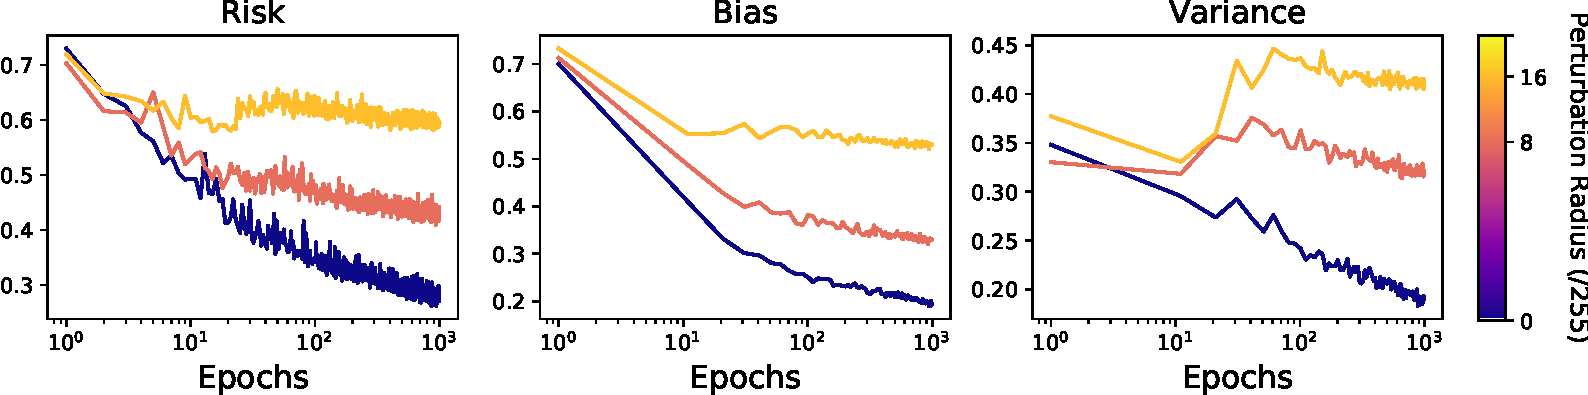
\includegraphics[width=0.95\textwidth]{figures/reason-variance.pdf}
%   \caption{``Risk'' (Average test error over independent training subsets) obtained when training on an adversarially augmented dataset, as well as the ``Bias'' and ``Variance'' following a bias-variance decomposition of the 0-1 loss. Detailed experiment settings can be found in Appendix~\ref{sect: exp-ad-augment}.
%   }
% \label{fig:dependence-variance}
% \end{figure*}




% Finally, we note that our above analyses echo the existing works. 
% Since implicit label noise modulates the double descent, and by Theorem~\ref{theo:label-noise-perturbation} it depends on the perturbation radius and data quality, the double descent in adversarial training should strongly correlate with the perturbation radius and data quality. Indeed, it has been observed respectively that small perturbation radius will not induce robust overfitting~\citep{Dong2021ExploringMI}, and high-quality data will not induce robust overfitting~\citep{Dong2021DataPF}.
% for small perturbation radius and high-quality dataset, the double descent may not be observed in adversarial training, which echos the recent empirical observation made in \citet{Dong2021ExploringMI} and \citet{Dong2021DataPF} respectively.
% \section{Mitigate Double Descent in Adversarial Training from the Implicit Label Noise Perspective}
\section{Mitigate Label Noise in Adversarial Training}
\label{sect:mitigate-double-descent}

% To mitigate the label noise in adversarial training, we focus on suppressing the implicit label noise from both theoretical and practical perspectives. 
Since the label noise is incurred by the mismatch between the true label distribution and assigned label distribution of adversarial examples in the training set, we wish to find an alternative label (distribution) for the adversarial example to reduce such distribution mismatch.
% \chengyu{But why this is better than the assigned distribution? Because the distribution mismatch is lower bounded by a positive, while here the mismatch can converge to $0$ as long as Lipschitz is sufficiently small.}
% Our goal is to construct an adversarially augmented dataset $\mathcal{D'}$ which contains little or no label noise.
% We've already shown that the predictive label distribution of a classifier trained on the conventional adversarially augmented dataset $\mathcal{D'} = \{(x', \tilde{y}'=\tilde{y})\}$, which we denote as \emph{model probability} in the following discussion, can in fact approximate the true label distribution. 
We've already shown that the predictive label distribution of a classifier trained by conventional adversarial training, which we denote as \emph{model probability} in the following discussion, can in fact approximate the true label distribution. 
Here we show that it is possible to further improve the predictive label distribution and reduce the label noise by calibration.
    
% Since the double descent is mainly caused by the mismatch between the assigned label and true label distributions and also the true label distribution is missing in most of real-world datasets, we propose to approximate the true label distribution.

% \subsection{Approximate the true label distribution}
% --- This previous title feels like we need true label distribution
\subsection{Rectify model probability to reduce distribution mismatch}
% \subsection{Calibrated model probability as adversarial labels}
% approximate the true label distribution}
\label{sect:approximate-true-distribution}





% \sout{We have shown that the double descent in adversarial training is due to the mismatch between the true label distribution and the assigned label distribution, which implicitly introduces label noise and promotes variance.} 
% \sout{A straightforward solution to double descent is thus to employ the true label distribution into training, based on which the label of the adversarial example can be sampled.
% However, since the perturbation radius allowed in adversarial training is typically small, the distribution mismatch might not be reflected by hard-label sampling if the training set is not sufficiently large. 
% To overcome this problem without significantly augmenting the training set, one can directly employ the true label distribution into the training objective.} 
% \sout{For cross-entropy loss it is easy to prove that the training objective with soft-label supervision is equivalent to that with hard labels sufficiently sampled based on the corresponding label distribution, namely}~\footnote{It is worth mentioning that $x$ in this section could either be a clean example or adversarial example. We therefore do not distinguish for simplicity.}
% \begin{equation}
%     \label{eq:loss-soft-label}
%     \mathbbm{E}_{(x, y) \sim p(x, y)} \ell(f(x; \theta), y) = \mathbbm{E}_{x \sim p(x)} \ell(f(x; \theta), p(y|x)).
% \end{equation}

    % \begin{theorem}[Error induced by an approximate label distribution]
    % \label{theorem: loss-error}
    % Let $\tilde{p}(y|x)$ be an approximation of $p(y|x)$, we have
    % \begin{equation}
    %     \ell(f(x;\theta), \tilde{p}) \le \ell(f(x;\theta), p) + 2 \left\|\tilde{p} - p\right\|_{TV} \left\|\log f(x; \theta)\right\|_1,
    % \end{equation}
    % where we neglect the expectation for simplicity. \jingbo{we may want to directly define the loss based on the label distribution as a weighted sum.}
    % \end{theorem}
    % It is worth mentioning that $x$ and $y$ here can be either a clean example or a adversarial example. 
    % One can simply replace them by $x + \delta$ and $y_\delta$ and the conclusion will still hold.
    % We therefore do not distinguish for simplicity.
    
    
% \note{We believe model probability can approach the true label distribution better than the assigned label} \chengyu{need this sentence as the next Section hasn't experiment on temperature and ratio yet. Or we have to emphasize in next section the optimal temperature is already 1.0!}




% \chengyu{We now wish to find such an assigned label of adversarial example such it is closer to the true label distribution $p_\theta(y_\delta | x)$}

%% -- Do Not Delete! -- \note{Problem of using calibration: validation set is not always available in practice. If a validation set is readily available, we can just use early stopping. Solution: We can also use other calibration methods without the need of a validation set, like learning well-calibrated confidence during training.}
%% --------------------

We show that it is possible to reduce the distribution mismatch by \emph{temperature scaling}~\citep{Hinton2015DistillingTK, Guo2017OnCO} enabled in the softmax function.
% We show that it is possible to reduce the distribution mismatch by utilizing the predictive probability of a classifier trained on traditional adversarial labels, which we refer as the \emph{model probability} for simplicity.
% % We denote the predictive probability of a classifier trained based on traditional adversarial labels as \textbf{model probability}. 
% We provide a theoretical guarantee to show that, with \emph{temperature scaling}~\citep{Hinton2015DistillingTK, Guo2017OnCO} enabled in the softmax function, model probability induces a distribution mismatch provably smaller than the traditional adversarial label.
% \note{Need another assumption here such the original label distribution is almost one-hot.} Given in notation section
% \begin{theorem}[Model probability induces smaller distribution mismatch than the traditional adversarial label]
\begin{theorem}[Temperature scaling can reduce the distribution mismatch]
\label{theorem: model-probability}
% \todo{Before we already show that robust model can learn the true label distribution. It is thus natural to use model probability as surrogate assigned label. Here we just need to show with temperature $T$ it can be better.}
    % Let $\mathbbm{1}(\hat{y})$ denote the one-hot vector of a label $\hat{y}$.
    Let $f_\theta(x; T)$ denote the predictive probability of a probabilistic classifier scaled by temperature $T$, namely $f_\theta(x; T)_j = \exp(z_j/T) / (\sum_j \exp(z_j / T)), $
    % $$
    %     f_\theta(x; T)_j = \frac{\exp(z_j/T)}{\sum_j \exp(z_j / T)},
    % $$
    where $z$ is the logits of the classifier from $x$. 
    Let $x'$ be an adversarial example correctly classified by a classifier $f_\theta$, i.e. $\argmax_j f_\theta(x')_j = y'$,
    % Assume the classifier can correctly classify an adversarial example $x_\delta$, i.e. $\argmax_j f(x_\delta; \theta, T)_j = p^*_\delta$,
    then there exists $T$, such that
    $$
    % \| f(x_\delta; \theta, T) - p(y^*_\delta|x) \|_{TV} \le \| \mathbbm{1}(\hat{y}) - p\|_{TV}.
    % \| f_\theta(x_\delta; T) - P(Y^*_\delta|x_\delta) \|_{TV} \le \| P(\tilde{Y}_\delta | x_\delta) - P(Y^*_\delta | x_\delta)\|_{TV}.
    \| f_\theta(x'; T) - P(Y'|x') \|_{TV} \le \| f_\theta(x') - P(Y' | x')\|_{TV}.
    $$

    % where $\mathbbm{1}(\hat{y})$ is the one-hot vector of $\hat{y}$.
\end{theorem}

% \todo{Replace the definition of traditional adversarial label  by the distribution of clean input directly.}


    Another way to further reduce the distribution mismatch is to interpolate between the model probability and the one-hot assigned label.
    % the traditional adversarial label. 
    We show that the interpolation works specifically for incorrectly classified examples and thus can be viewed as a complement to temperature scaling.
    \begin{theorem}[Interpolation can further reduce the distribution mismatch]
    \label{theorem: model-probability-coefficient}
    % \chengyu{Will it be a problem if $y$ is now no longer the argmax?}
        % Assume the classifier $f$ incorrectly classify an adversarial example $x_\delta$, i.e. $\argmax_j f(x_\delta; \theta)_j \ne p^*_\delta$.
        Let $x'$ be an adversarial example incorrectly classified by a classifier $f_\theta$, i.e. $\argmax_j f_\theta(x'; T)_j \ne y'$. % \argmax_j p(y=j|x)$. 
        % Assume $\hat{y} = \argmax_j~p(y=j|x)$ and $\max_j p(y=j|x) \ge 1/2$, then there exists $\lambda$, such that
        Assume $\max_j P(Y'=j|x') \ge 1/2$, then there exists an interpolation ratio $\lambda$, such that
        \begin{equation*}
        \small
        % \|  P_{\theta}^{T, \lambda}(Y'|x') - P(Y' | x') \|_{TV} \le \| f_\theta(x_\delta; T) - P(Y_\delta^* | x_\delta)\|_{TV},  
         \| f_\theta(x'; T, \lambda) - P(Y' | x') \|_{TV} \le \| f_\theta(x'; T) - P(Y' | x')\|_{\text{TV}},
        \normalsize
        \end{equation*}
        where $f_\theta(x'; T, \lambda) = \lambda \cdot f_\theta(x'; T) + (1 - \lambda)\cdot P(\tilde{Y}' | x')$.
        % where $P_{\theta}^{T, \lambda}(Y_\delta|x_\delta) = \lambda \cdot f_\theta(x_\delta; T) + (1 - \lambda)\cdot P(\tilde{Y}_\delta | x_\delta) $.
        % \jingbo{Also, did you forget the include $T$ in $f$?}\chengyu{This theorem should work for any $T$, so i neglect it.}
    \end{theorem}
    % Note the above theorem focus on incorrectly classified examples and thus can be regarded as a complement to Theorem~\ref{theorem: model-probability}.
    % We show that a proper interpolation approximates provably better for incorrectly classified examples, therefore this theorem can be regarded as a complement to the above one.
    
    
    As a summarization, 
    % an potentially better approximation of the true label distribution based on a model can be formulated as
    to reduce the distribution mismatch, we propose to use 
    $f_\theta(x'; T, \lambda)$
    % $P_{\theta}^{T, \lambda}(Y_\delta|x_\delta)$ 
    % following distribution 
    as the assigned label of the adversarial example in adversarial training, which we refer as the \emph{rectified model probability}.
    % \begin{equation}
    %     \label{eq:approximate-label-distribution}
    %     P_{\theta}^{T, \lambda}(Y_\delta|x_\delta) = \lambda \cdot f_\theta(x_\delta; T) + (1- \lambda) \cdot P(\tilde{Y}_\delta | x_\delta),
    % \end{equation}
    % We refer this label distribution as the \textbf{rectified model probability}.
    
    In Appendix~\ref{sect:optimal-temperature-mixup}, we show that the optimal hyper-parameters (i.e. $T$ and $\lambda$) of almost all training examples concentrate on the same set of values by studying on a synthetic dataset with known true label distribution. 
    % \jingbo{can we name the values here?}
    Therefore it is possible to find an universal set of hyper-parameters that reduce the distribution mismatch for all adversarial examples. 
    % the rectified model probability can often approximate the true distribution sufficiently well with



version https://git-lfs.github.com/spec/v1
oid sha256:fc01b3c0a6353e705e9d70f0e94f348c47073c0d6ebf49c38c83cccabcc985f0
size 5193

version https://git-lfs.github.com/spec/v1
oid sha256:8d5c41dc9086b855877de17136ceee40552d38dd2e6697de9ec78de32b4c4161
size 2079

\section{Experiments}
\label{sect:experiment}

\FloatBarrier










% \begin{table*}[!ht]
%   \small
%   \caption{Performance of our method combined with SWA and an additional standard teacher. %  on different datasets.
%   }
%   \vspace{0.5ex}
%   \label{table:result-technique}
%   \centering
%   \small
%   \begin{tabular}{clcccccccc}
%     \toprule
%     \multirow{2}{*}{Dataset} & \multirow{2}{*}{Setting} & \multirow{2}{*}{$T$} & \multirow{2}{*}{$\lambda$} & \multicolumn{3}{c}{Robust Acc. (\%)} & \multicolumn{3}{c}{Standard Acc. (\%)}\\
%      & & &  & Best & Last & Diff. & Best & Last & Diff.\\
%     \midrule
%     % \multirow{3}{*}{CIFAR-10} 
%     % & AT & - & - &  $47.35$ & $41.42$ & $ 5.93$ &  $82.67$ &  $84.91$ & -$2.24$ \\
%     % &  KD-AT + KD-Std + SWA & $2$ & $0.5$ & $49.98$ & $49.89$ & $0.09$ & $\textbf{85.06}$ & $\textbf{85.52}$ & -$0.46$\\
%     % & KD-AT-Auto + KD-Std + SWA & $1.47^*$ & $0.8^*$ & $\textbf{50.03}$ & $\textbf{50.05}$ & $\textbf{-0.02}$ & $84.69$ & $84.91$ & $\textbf{-0.22}$\\ 
%     %     \midrule
%     \multirow{3}{*}{SVHN} 
%     & AT & - & - & $47.83$ & $39.77$ & $8.06$ & $90.18$ & $91.11$ & -$0.93$\\
%     & KD-AT + KD-Std + SWA & $2$ & $0.5$ & $47.88$ & $46.46$ & $1.42$ & $\textbf{91.59}$ & $\textbf{91.76}$ & $\textbf{-0.17}$\\
%     & KD-AT-Auto + KD-Std + SWA  & $1.53^*$ & $0.83^*$ & $\textbf{50.58}$ & $\textbf{50.09}$ & $\textbf{0.49}$ & $90.54$ & $90.76$ & -$0.22$\\ 
%     \bottomrule
%     % \tablefootnote{$^*$ indicates the best hyper-parameter searched.}
%   \end{tabular}
% \end{table*}





% \note{Should describe our method again as a whole again? Maybe discuss the difference between our work and Chen et al in more detail in the related work. We further calibrate their method to achieve even smaller overfitting w/o additional human effort.}
% \note{So Why not SWA? Why not clean teacher? Not convenient? Focus on ad training?}
% \chengyu{This section extends to other settings, therefore an independent section}.


% \chengyu{Possible names of methods
% \note{KD-AT}
% \note{AKD-AT (Adaptive knowledge distillation)}
% \note{LabelRectifier}
% \note{Rectified }
% }

% In this section, we verify the effectiveness of our method on multiple datasets. 


\begin{figure*}[t]
  \centering
  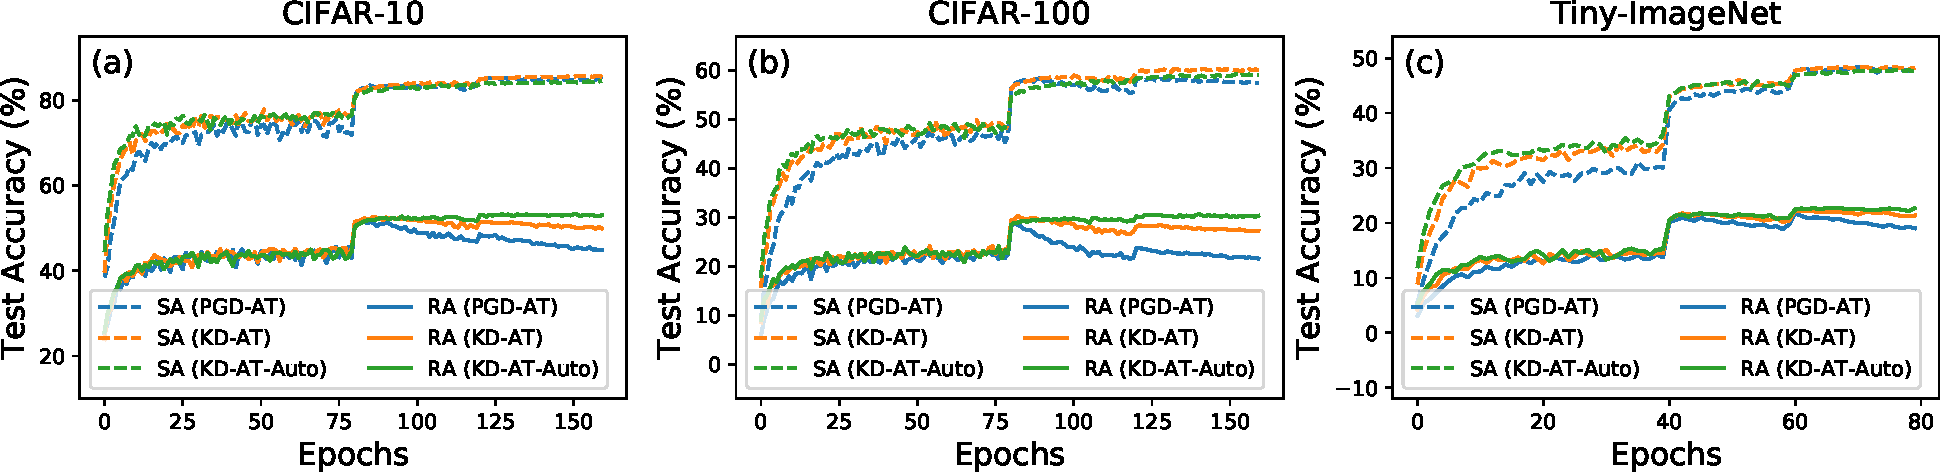
\includegraphics[width=0.98\linewidth]{figures/mitigate-overfitting.pdf}
  \vspace{-1ex}
  \caption{Our method can effectively mitigate robust overfitting for different datasets. 
  }
\label{fig:mitigate-overfitting}
% \vspace{-2ex}
\end{figure*}

% \jingbo{it's a bit odd to me to put the figure in the beginning of a section. }

\smallsection{Experiment setup}
We conduct experiments on three datasets including CIFAR-10, CIFAR-100~\citep{Krizhevsky2009LearningML} and Tiny-ImageNet~\citep{Le2015TinyIV}. We conduct PGD training on pre-activation ResNet-18~\citep{He2016IdentityMI} with $10$ iterations and perturbation radius $8/255$ by default. We evaluate robustness against $\ell_\infty$ norm-bounded adversarial attack with perturbation radius $8/255$, and employ AutoAttack~\citep{Croce2020ReliableEO} for reliable evaluation.  
% We employ SGD as the optimizer with momentum and weight decay set as $0.9$ and $0.0005$ respectively. We conduct the training for $160$ epochs with the learning rate starting at $0.1$ and reduced by a factor of $10$ at epoch $80$ and $120$.
Appendix~\ref{sect:more-result} includes results on additional model architectures (e.g., VGG~\citep{Simonyan2015VeryDC}, WRN),  adversarial training methods (e.g., TRADES~\citep{Zhang2019TheoreticallyPT}, FGSM~\citep{Goodfellow2015ExplainingAH}), and evaluation metrics (e.g., PGD-1000 (PGD attack with $1000$ iterations), Square Attack~\citep{Andriushchenko2020SquareAA}, RayS~\citep{Chen2020RaySAR}). More setup details can be found in Appendix~\ref{sect:exp-setting-all}.

% as an example and include results on TRADES~\citep{Zhang2019TheoreticallyPT} and FGSM~\citep{Goodfellow2015ExplainingAH} in Appendix~\ref{sect:more-result}.  
% The results against more evaluation metrics such as PGD-$1000$ (PGD attack with $1000$ iterations), Square Attack~\citep{Andriushchenko2020SquareAA} and RayS~\citep{Chen2020RaySAR} will be provided in Appendix~\ref{sect:more-result}. 
% We choose pre-activation ResNet-18~\citep{He2016IdentityMI} in the main paper and experiment on more architectures including VGG~\citep{Simonyan2015VeryDC} and WRN in Appendix~\ref{sect:more-result}.



% -------------- Dataset ----------------
\begin{table*}[!t]
  \small
  \caption{Performance of our method on different datasets. $^*$ denotes the hyper-parameters automatically determined by our method. % \chengyu{Results on SVHN. Figure too?}
   }
  \vspace{0.5ex}
  \label{table:result-dataset}
  \centering
  \small
  \begin{tabular}{clcccccccc}
    \toprule
    \multirow{2}{*}{Dataset} & \multirow{2}{*}{Setting} & \multirow{2}{*}{$T$} & \multirow{2}{*}{$\lambda$} & \multicolumn{3}{c}{Robust Acc. (\%)} & \multicolumn{3}{c}{Standard Acc. (\%)}\\
     & & &  & Best & Last & Diff. & Best & Last & Diff.\\
    \midrule
\multirow{3}{*}{CIFAR-10} 
& AT & - & - &  $47.35$ & $41.42$ & $ 5.93$ &  $82.67$ &  $84.91$ & -$2.24$ \\
 & KD-AT & $2$ & $0.5$ &  $48.76$ & $46.33$ & $ 2.43$ &  $82.89$ &  $\textbf{85.49}$ & -$2.60$ \\ 
 & KD-AT-Auto & $1.47^*$ & $0.8^*$ &  $\textbf{49.05}$ & $\textbf{48.80}$ & $ \textbf{0.25}$ &  $\textbf{84.26}$ &  $84.47$ & $\textbf{-0.21}$ \\ 
    \midrule
\multirow{3}{*}{CIFAR-100}
& AT & - & - &  $24.79$ & $19.75$ & $ 5.04$ &  $57.33$ &  $57.42$ & -$0.09$ \\ 
& KD-AT & $2$ & $0.5$ &  $25.77$ & $23.58$ & $ 2.19$ &  $57.24$ &  $\textbf{60.04}$ & -$2.80$ \\ 
& KD-AT-Auto & $1.53^*$ & $0.83^*$ &  $\textbf{26.36}$ & $\textbf{26.24}$ & $\textbf{0.12}$ &  $\textbf{58.80}$ &  $59.05$ & $\textbf{-0.25}$ \\ 
\midrule
\multirow{3}{*}{Tiny-ImageNet} 
& AT & - & - &  $17.20$ & $15.40$ & $ 1.80$ &  $47.72$ &  $47.62$ & $ 0.10$ \\ 
& KD-AT & $2$ & $0.5$ &  $17.86$ & $17.18$ & $ 0.68$ &  $\textbf{47.73}$ &  $\textbf{48.28}$ & -$0.55$ \\ 
& KD-AT-Auto  & $1.23^*$ & $0.85^*$ &  $\textbf{18.29}$ & $\textbf{18.39}$ & $\textbf{-0.10}$ &  $47.46$ &  $47.56$ & $\textbf{-0.10}$ \\ 
    \bottomrule
    % \tablefootnote{$^*$ indicates the best hyper-parameter searched.}
  \end{tabular}
\end{table*}
% \vspace{-1.5em}


\smallsection{Results \& Discussions}
Our method is essentially the baseline adversarial training with a robust-trained self-teacher, equipped with an algorithm automatically deciding the optimal hyper-parameters, which we now denote as KD-AT-Auto.
We compare KD-AT-Auto with two baselines: regular adversarial training (AT), and adversarial training combined with self-distillation (KD-AT) with fixed temperature $T=2$ and interpolation ratio $\lambda=0.5$ as suggested by \citet{chen2021robust}. 

As shown in Figure~\ref{fig:mitigate-overfitting}, our method can effectively mitigate robust overfitting for all datasets, with both standard accuracy (SA) and robust accuracy (RA) constantly increasing throughout training. In Table~\ref{table:result-dataset}, we measure the difference between the RA at the best checkpoint (Best) and at the last checkpoint (Last) to clearly show the overfitting gap. Our method can reduce the overfitting gap to less than $0.5\%$ for all datasets. One may note that self-distillation with fixed hyper-parameters is in fact inferior in terms of reducing robust overfitting, while its effectiveness can be significantly improved with the optimal hyper-parameters automatically determined by our method, which further verifies our understanding of robust overfitting. 
Compared with self-distillation with fixed hyper-parameters, our method can also boost both RA and SA at the best checkpoint for all datasets.


Our method can further be combined with orthogonal techniques such as Stochastic Weight Averaging (SWA)~\citep{Izmailov2018AveragingWL} and additional standard teachers as mentioned in previous work~\citep{chen2021robust} to achieve better performance. More results and discussion can be found in Appendix~\ref{sect:additional-technique}.


% \note{One thing is not doing good is the last standard acc.}


    % We note that employing Equation~(\ref{eq:approximate-label-distribution}) as the supervision in adversarial training with cross-entropy loss is equivalent to the self-training method proposed by~\citet{chen2021robust} without a standard-trained teacher\footnote{We find the standard-trained teacher does not help mitigate the robust overfitting, but rather improve the standard accuracy following a regular knowledge distillation practice.}. 
    % However, the temperature $T$ and the interpolation ratio $\lambda$ have to be manually set in the self-training method, whereas they can be automatically tuned in our method. Figure~\ref{fig:mitigate-overfitting} shows that our automatically-tuned can reduce the overfitting gap better than the fixed hyperparameters for a variety of datasets.
    
    
% \subsection{Combined with additional orthogonal techniques}
% \label{sect:additional-technique}

% Our method can further be combined with other orthogonal techniques such as Stochastic Weight Averaging (SWA)~\citep{Izmailov2018AveragingWL} and additional standard teachers as mentioned in previous work~\citep{chen2021robust} to achieve better performance. 

% More results and discussion can be found in Appendix~\ref{sect:additional-technique}.

% Here, we show that combined with the additional techniques proposed in~\citep{chen2021robust}, our method can achieve better performance.

% We note that our proposed method is essentially the baseline knowledge distillation for adversarial training with a robustly trained self-teacher, equipped with an algorithm that automatically finds its optimal hyperparameters (i.e. the temperature $T$ and the interpolation ratio $\lambda$). Stochastic Weight Averaging (SWA) and additional standard teachers employed in~\citep{chen2021robust} are orthogonal contributions. KD-AT-Auto can certainly be combined with SWA and KD-Std to achieve better performance. 

% We note that the method proposed by \citet{chen2021robust}, namely combining knowledge distillation with self-distillation, an additional standard teacher and SWA (KD-AT + KD-Std + SWA), can already reduce the overfitting gap to almost $0$. It is thus hard to see any further reduction by combining our method. To this end, we introduce an extra dataset SVHN~\citep{Netzer2011ReadingDI}. As shown in Table~\ref{table:result-technique}, on SVHN, the above method KD-AT + KD-Std + SWA still produces a high overfitting gap (also see Appendix A1.3 in~\citep{chen2021robust}), whereas by combining with our method (KD-AT-Auto + KD-Std + SWA), the overfitting gap can be further reduced to almost $0$. This demonstrates the advantage of our principle-guided method on mitigating robust overfitting. More results regarding other datasets and detailed experiment setup can be found in Appendix~\ref{sect:additional-technique}.

% As shown in Table~\ref{table:result-technique}, on CIFAR-10, KD-AT + KD-Std + SWA~\citep{chen2021robust} can already reduce the overfitting gap (difference between the best and last robust accuracy) to almost 0, while KD-AT-Auto + KD-Std + SWA maintains an overfitting gap close to 0. Interestingly, on the SVHN dataset~\citep{Netzer2011ReadingDI}, where KD-AT + KD-Std + SWA still produces a high overfitting gap (also see Appendix A1.3 in~\citep{chen2021robust}), KD-AT-Auto + KD-Std + SWA can further push this gap to close to 0. 

% Here, the interpolation ratio of the standard teacher is fixed as $0.2$ and the SWA starts at the first learning rate decay for all experiments. We employ PGD-AT~\citep{Madry2018TowardsDL} as the base adversarial training method and conduct experiments with a pre-activation ResNet-18. The robust accuracy is evaluated with AutoAttack. Other experiment details are in line with Appendix~\ref{sect: exp-practical}.


% Furthermore, we note that~\citep{chen2021robust} shows SWA and KD-Std are essential components to mitigate robust overfitting on top of KD-AT, while we show that KD-AT itself can mitigate robust overfitting by proper parameter tuning. We are thus able to separate these components and allow a more flexible selection of hyperparameters in diverse training scenarios without fear of overfitting. In particular, although~\citep{chen2021robust} suggests SWA starting at the first learning rate decay (exactly when the overfitting starts) mitigates robust overfitting, the effectiveness of SWA on mitigating overfitting may strongly depend on its hyper-parameter selection including $s_0$, i.e., the starting epoch and $\tau$, i.e., the decay rate\footnote{SWA can be implemented using an exponential moving average $\theta'$ of the model parameters $\theta$ with a decay rate $\tau$, namely $\theta' \leftarrow \tau \cdot \theta' + (1-\tau) \cdot \theta$ at each training step~\citep{Rebuffi2021FixingDA}.}, which is also mentioned in recent work~\citep{Rebuffi2021FixingDA}. We also did some additional experiments on CIFAR-10 following the SWA setting in~\citep{Rebuffi2021FixingDA} to demonstrate the wide applicability of our method. As shown by Table~\ref{table:result-swa}, when changing the hyperparameters of SWA, KD-AT + KD-Std + SWA cannot consistently mitigate robust overfitting, while KD-AT-Auto + KD-Std + SWA can maintain an overfitting gap close to 0 and achieve better robustness as well. 



\section{Conclusion and Discussions}
\label{sect:conclusion}

% \chengyu{if no size, remove all equation number}

In this paper, we show that label noise exists implicitly in adversarial training due to the mismatch between the true label distribution and the assigned label distribution of adversarial examples. Such label noise can explain the dominant overfitting phenomenon. Based on a label noise perspective, we also extend the understanding of robust overfitting and show that it is the early part of an epoch-wise double descent in adversarial training. Finally, we propose an alternative labeling of adversarial examples by rectifying model probability, which can effectively mitigate robust overfitting without any manual hyper-parameter tuning. 
% Our further analyses show that the double descent may originate from the implicit label noise introduced by the improper labeling of the adversarial examples. Based on our understanding, we propose an alternative labeling of adversarial examples by rectifying model probability, which can effectively mitigate robust overfitting without any manual hyper-parameter tuning. 
% \jingbo{this without hyper-parameter tuning reads odd to me. Maybe say without manual tuning?}
% In the future, we also plan to explore if it is possible to rectify the model probability on the fly during the adversarial training for a better efficiency.

The label noise implicitly exists in adversarial training may have other important effects on adversarially robust learning. This can potentially consolidate the theoretical grounding of robust learning. For instance, since label noise induces model variance, from a model-wise view, one may need to increase model capacity to reduce the variance. This may partially explain why robust generalization requires significantly larger model than standard generalization. 
% achieved by adversarial training is still significantly lower than the accuracy. One often has to greatly increase model capacity 

% our definition of implicit label noise from a distribution mismatch perspective may also exist in a variety of scenarios, especially in real-world tasks where labeling is often complicated and ambiguous. Our method to rectify such label noise should thus be applicable as well. This would be an interesting future work. 


% By showing robust overfitting and epoch-wise double descent are in fact the same phenomena, our work eases the difficulty in understanding overfitting in modern generalization theory. Existing theories on double descent can be readily applied to adversarially robust learning, and potentially consolidate the theoretical grounding of robust learning.



% \note{Since unify the two phenomena, we can deal with one. Theoretically we don't have to invent theory for robust overfitting, But just have to explore double descent in adversarial training.  And more specifically we can focus on dealing with the label noise induced by distribution mismatch.}

% \note{Remove this if no space left.}
% Beyond the double descent in adversarial training, our definition of implicit label noise from a distribution mismatch perspective may also exist in a variety of scenarios, especially in real-world tasks where labeling is often complicated and ambiguous. Our method to rectify such label noise should thus be applicable as well. This would be an interesting future work. 

% Can broadly benefit similar overfitting case
% - Label noise \#TODO
% - Ambiguity in text?
% - Image classification with multiple objects (classification without detection?)

% from a hard-label mismatch to a distribution mismatch, thus enabling a wide variety of approaches to observe double descent in modern learning practice including the adversarial augmentation and mixup augmentation mentioned in the paper other than adversarial training. On the other hand, Gaussian noise and other common corruptions~\citep{Hendrycks2019BenchmarkingNN}, which does not cause distribution mismatch, have been shown to fail to produce double descent~\citep{Yang2020RethinkingBT}. These empirical observations suggest there is a deeper connection between implicit label noise and double descent in classification problems, where the theoretical progress still lags behind.

% \note{thus offer a theoretical playground for analyzing the label noise in classification problems. Currently still rely on label flipping noise and some feature noise}

% -- Finally, on the practical side, our understanding of robust overfitting opens new opportunities to advance adversarial training practice. Better labeling of the adversarial examples may be still in demand to further reduce robust overfitting.

% Techniques that have been shown to improve the uncertainty quality of the model probability such as ensembles~\citep{Lakshminarayanan2017SimpleAS} can further mitigate the double descent and improve adversarial robustness. 
% Meanwhile, we note that an alternative labeling not necessarily has to be obtained from a surrogate model, but can also be based on the model itself during training, which can minimize the computation overhead and is more suitable for practical deployment of adversarial training methods. Strategies in this vein have already demonstrated their effectiveness on mitigating robust overfitting~\citep{Huang2020SelfAdaptiveTB}. % Following this idea, a group of strategies succeeding in conventional noisy learning is known as \emph{bootstrapping}~\citep{Reed2015TrainingDN, Sanchez2019UnsupervisedLN, Huang2020SelfAdaptiveTB}, where the last work already demonstrated the effectiveness of their method on adversarial training.




% * Potential explanation to knowledge distillation

% * kd should also be useful in label noise, interesting no work use this, currently people use a small clean data
% \citep{Li2017LearningFN, Zhang2020DistillingES}.

% \clearpage
% \newpage

% \section*{Reproduciblity Statement}

% We conduct experiments on public benchmark. 
% We will release implementations for all methods and scripts for all experiments on GitHub, under the Apache-2.0 license.

% \section*{Ethic Statement}

% In this paper, we explore the double descent phenomenon in adversarial robust learning from the implicit label noise perspective.
% We experiment on three benchmark datasets that are publicly available.
% Our analyses offer more in-depth understandings about adversarial training and can better improve the robustness of neural network models.
% Therefore, we believe our work is ethically on the right side of spectrum and has no potential for misuse, and cannot harm any vulnerable population.


% \newpage
\bibliography{icml2022}
\bibliographystyle{icml2022}

% \newpage
%%%%%%%%%%%%%%%%%%%%%%%%%%%%%%%%%%%%%%%%%%%%%%%%%%%%%%%%%%%%
\section*{Checklist}


%%% BEGIN INSTRUCTIONS %%%
The checklist follows the references.  Please
read the checklist guidelines carefully for information on how to answer these
questions.  For each question, change the default \answerTODO{} to \answerYes{},
\answerNo{}, or \answerNA{}.  You are strongly encouraged to include a {\bf
justification to your answer}, either by referencing the appropriate section of
your paper or providing a brief inline description.  For example:
\begin{itemize}
  \item Did you include the license to the code and datasets? \answerYes{See Section~\ref{gen_inst}.}
  \item Did you include the license to the code and datasets? \answerNo{The code and the data are proprietary.}
  \item Did you include the license to the code and datasets? \answerNA{}
\end{itemize}
Please do not modify the questions and only use the provided macros for your
answers.  Note that the Checklist section does not count towards the page
limit.  In your paper, please delete this instructions block and only keep the
Checklist section heading above along with the questions/answers below.
%%% END INSTRUCTIONS %%%


\begin{enumerate}


\item For all authors...
\begin{enumerate}
  \item Do the main claims made in the abstract and introduction accurately reflect the paper's contributions and scope?
    % \answerTODO{}
    \answerYes{}
  \item Did you describe the limitations of your work?
    % \answerTODO{}
    \answerYes{See Section~\ref{sect:limitation}}
  \item Did you discuss any potential negative societal impacts of your work?
    % \answerTODO{}
    \answerYes{See Section~\ref{sect:limitation}}
  \item Have you read the ethics review guidelines and ensured that your paper conforms to them?
    % \answerTODO{}
    \answerYes{}
\end{enumerate}


\item If you are including theoretical results...
\begin{enumerate}
  \item Did you state the full set of assumptions of all theoretical results?
    % \answerTODO{}
    \answerYes{}
        \item Did you include complete proofs of all theoretical results?
    % \answerTODO{}
    \answerYes{}
\end{enumerate}


\item If you ran experiments...
\begin{enumerate}
  \item Did you include the code, data, and instructions needed to reproduce the main experimental results (either in the supplemental material or as a URL)?
    % \answerTODO{}
    \answerYes{}
  \item Did you specify all the training details (e.g., data splits, hyperparameters, how they were chosen)?
    % \answerTODO{}
    \answerYes{}
        \item Did you report error bars (e.g., with respect to the random seed after running experiments multiple times)?
    % \answerTODO{}
    \answerYes{}
        \item Did you include the total amount of compute and the type of resources used (e.g., type of GPUs, internal cluster, or cloud provider)?
    % \answerTODO{}
    \answerYes{}
\end{enumerate}


\item If you are using existing assets (e.g., code, data, models) or curating/releasing new assets...
\begin{enumerate}
  \item If your work uses existing assets, did you cite the creators?
    % \answerTODO{}
    \answerYes{}
  \item Did you mention the license of the assets?
    % \answerTODO{}
    \answerNA{}
  \item Did you include any new assets either in the supplemental material or as a URL?
    % \answerTODO{}
    \answerNA{}
  \item Did you discuss whether and how consent was obtained from people whose data you're using/curating?
    % \answerTODO{}
    \answerNA{}
  \item Did you discuss whether the data you are using/curating contains personally identifiable information or offensive content?
    % \answerTODO{}
    \answerNA{}
\end{enumerate}


\item If you used crowdsourcing or conducted research with human subjects...
\begin{enumerate}
  \item Did you include the full text of instructions given to participants and screenshots, if applicable?
    % \answerTODO{}
    \answerNA{}
  \item Did you describe any potential participant risks, with links to Institutional Review Board (IRB) approvals, if applicable?
    % \answerTODO{}
    \answerNA{}
  \item Did you include the estimated hourly wage paid to participants and the total amount spent on participant compensation?
    % \answerTODO{}
    \answerNA{}
\end{enumerate}


\end{enumerate}


%%%%%%%%%%%%%%%%%%%%%%%%%%%%%%%%%%%%%%%%%%%%%%%%%%%%%%%%%%%%


\newpage
\appendix\onecolumn
\section{Proofs}
\label{sect:proof-all}


\subsection{Preliminaries}
\smallsection{Proof in Assumption~\ref{assumption:clean-dataset}}
Here we prove that if there no label error in the clean dataset, then $P(\tilde{Y}|x) = P(Y|x)$.

\begin{proof}
First, we note that 
$$
    P(\tilde{Y}=j'|x) = \sum_j P(\tilde{Y}=j'| Y=j, x) P(Y=j|x).
$$
Since $P(E=1| Y=j, x) = 0$ we have,
$$
    \begin{aligned}
    P(\tilde{Y}=j'| Y=j, x)
    & = \sum_e P(\tilde{Y}=j'| E=e, Y=j, x) P(E=e| Y=j, x)  \\
    & = P (\tilde{Y}=j'| E=0, Y=j, x) \\
    & = 
    \begin{cases}
    1, & ~\text{if}~j'=j,\\
    0, & ~\text{otherwise}.
    \end{cases}
    \end{aligned}
$$
Therefore we have for all $j'$,
$$
    P(\tilde{Y}=j'|x) = P(Y=j'|x). 
$$
\end{proof}



\smallsection{Total Variation distance for discrete probability distributions}
    For two discrete probability distributions $P(Y)$ and $P(Y')$ where $Y, Y'\in\mathcal{Y}$, the total variation distance between them can be equally defined as
    $$
     \begin{aligned}
       \|P(Y) - P(Y')\|_{\text{TV}} 
       & = \sup_{J\in \mathcal{A}} \left| P(Y\in J) - P(Y'\in J)\right| \\
       & = \sup_{J\in \mathcal{A}} \left| \sum_{j\in J} P(Y=j) - \sum_{j\in J}P(Y'=j)\right| \\
      & = \frac{1}{2}\sum_j |P(Y=j) - P(Y'=j|)| \\
     \end{aligned}
    $$
     

version https://git-lfs.github.com/spec/v1
oid sha256:5dcbec9c39c036cca059d500cb9cd8d19febc02a840c7d02d19493040f0493d4
size 6551


version https://git-lfs.github.com/spec/v1
oid sha256:4c20a5b53d73abccb1fce4c76c5dece6f3aea2e8a55b7bc4e02c54d8f9e776c4
size 5859


version https://git-lfs.github.com/spec/v1
oid sha256:c1b6ee6986c75d24a1d6e66db5aad82072562a37af9cff13917d1ba3a4b01b54
size 5467

version https://git-lfs.github.com/spec/v1
oid sha256:0df0a5bf203733811ea888a1d46f8bdc8087b86bf6566202bea5d1b325066ef6
size 922

\section{More empirical analyses}

\subsection{Epoch-wise double descent is ubiquitous in adversarial training}
% \subsection{Reconcile robust overfitting and epoch-wise double descent}
\label{sect:double-descent-reconcile}

% In this section, we conduct extensive experiments with different optimizers, sample sizes, model architectures, and learning rate schedulers to verify the connection between robust overfitting and epoch-wise double descent. The default experiment settings are listed in Appendix~\ref{sect: exp-double-descent} in detail.

In this section, we conduct extensive experiments with different model architectures, and learning rate schedulers to verify the connection between robust overfitting and epoch-wise double descent. The default experiment settings are listed in Appendix~\ref{sect: exp-double-descent} in detail.


% We focus on PGD training as it is simple in nature and can produce robustness comparable to state-of-the-art methods~\cite{Rice2020OverfittingIA, pang2021bag, Gowal2020UncoveringTL}.

% \smallsection{Optimizer}
% Similar to the setting employed in \citet{Nakkiran2020DeepDD}, we conduct the adversarial training using both the Adam optimizer and SGD. As already shown in Figure~\ref{fig:intro}, double descent can be observed for both optimizers, although Adam may be inferior compared to SGD.


% \smallsection{Sample size}
% We randomly sample a desired number of examples without replacement from the original training set in CIFAR-10. As shown in Figure \ref{fig:reconcile-sample-size}, for both optimizers, increasing sample size will shrink the area under the double descent curve, but will not significantly distort its shape. 
% % reduce the overfitting gap, defined by the difference between the intermediate minimum and intermediate maximum of the robust test error.
% Similar observation is also made for double descent curve under standard training~\citep{Nakkiran2020DeepDD}.

% \begin{figure*}[!ht]
%   \centering
%   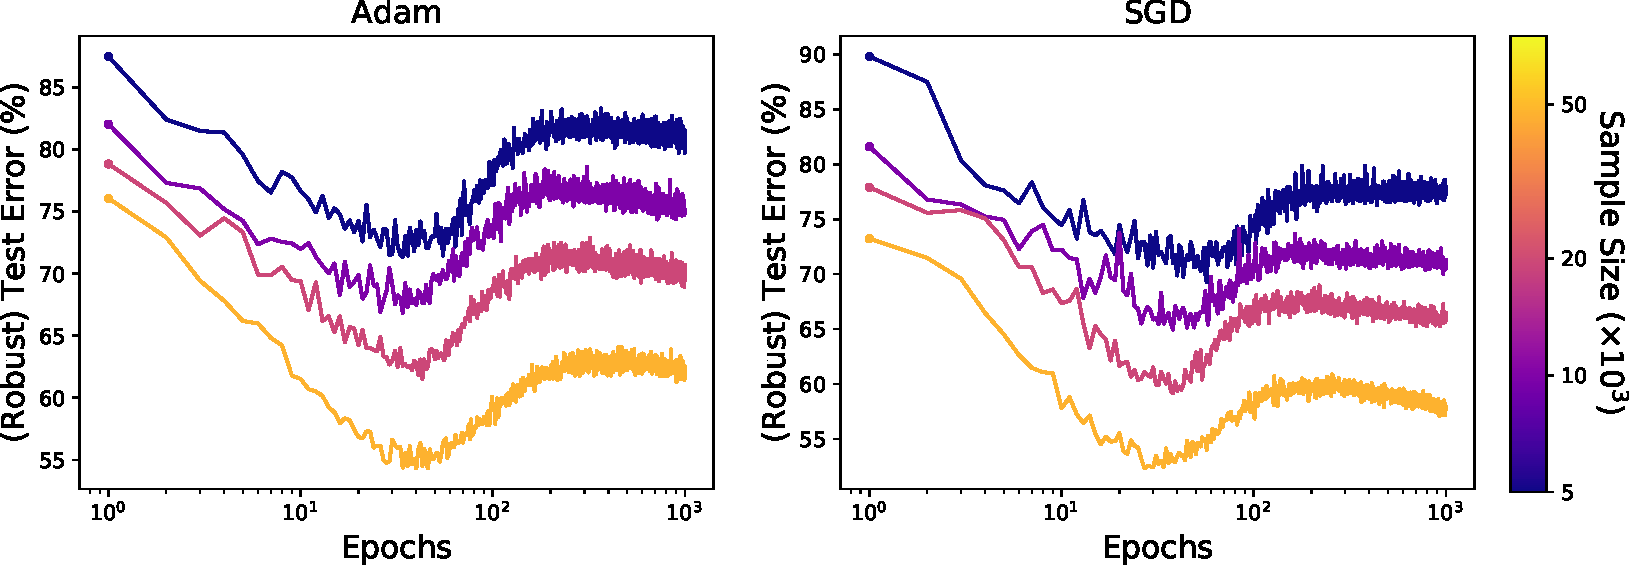
\includegraphics[width=0.9\textwidth]{figures/reconcile-sample-size.pdf}
%   \caption{Varying sample size will shrink the area under the epoch-wise double descent curve, but will not significantly distort its shape.
%   }
% \label{fig:reconcile-sample-size}
% \end{figure*}

% \subsection{Model, learning rate scheduler and regularization}

% \chengyu{Figure: Four subfigures side by side}


\smallsection{Model capacity}
We modulate the capacity of the deep model by varying the widening factor of the Wide ResNet. To extend the lower limit of the capacity, we allow the widening factor to be less than $1$. In such case, the number of channels in each residual block is scaled similarly but rounded, and the number of channels in the first convolutional layer will be reduced accordingly to ensure the width monotonically increasing through the forward propagation. 
% To accelerate the training with an extremely large model, we randomly sample a training set of size $5000$ and employ the Adam optimizer, since the sample size will not significantly distort the shape of the double descent as shown above. Figure~\ref{fig:reconcile-model-capacity} shows that the double descent will gradually become more complete as the model capacity increases and the model translates from under-parameterized to over-parameterized regime~\citep{Nakkiran2020DeepDD}.


\begin{figure*}[!ht]
\centering
\begin{subfigure}[t]{.48\textwidth}
  \centering
  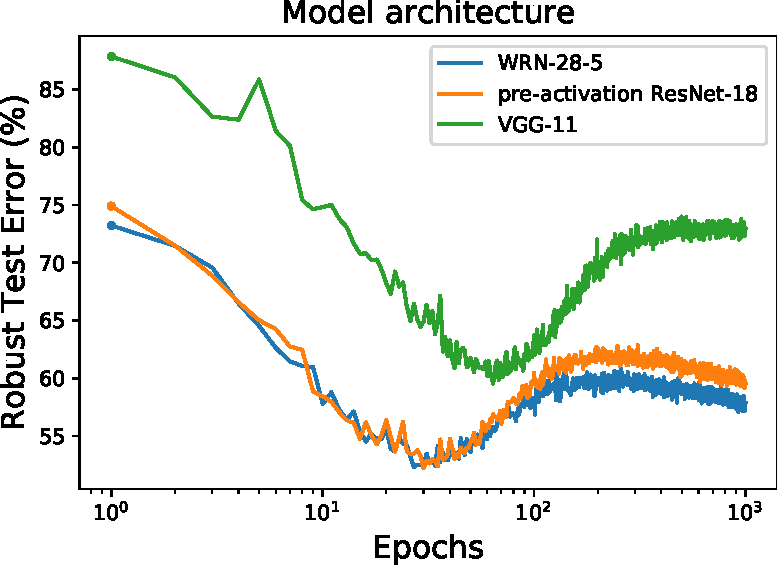
\includegraphics[width=.95\textwidth]{figures/reconcile-model-architecture.pdf}
  \caption{
  % Different model architectures will affect the double descent curve. In particular, VGG-11 will have the second descent delayed due to its inferior performance compared to residual architectures.
  Epoch-wise double descent curves in adversarial training with various model architectures.
  }
  \label{fig:reconcile-model-architecture}
\end{subfigure}\hfill
\begin{subfigure}[t]{.48\textwidth}
  \centering
  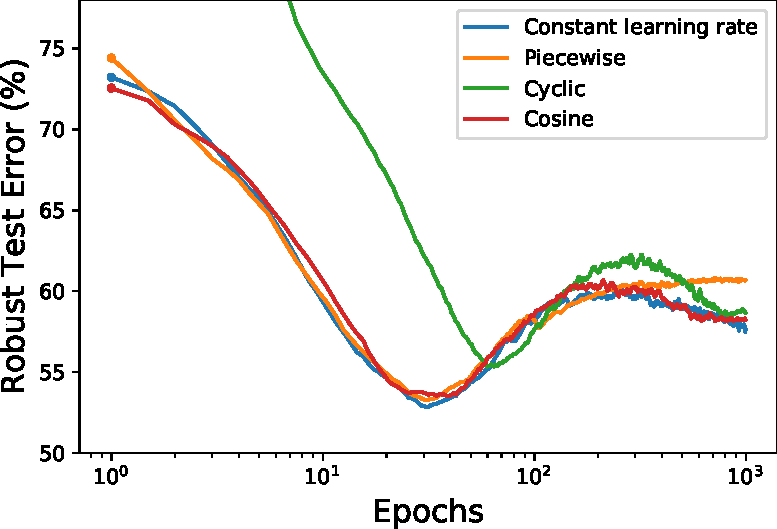
\includegraphics[width=0.95\textwidth]{figures/reconcile-lr-scheduler.pdf}
  \caption{
  % The effect of the learning rate scheduler on the epoch-wise double descent curve in adversarial training. Modulating the model capacity can produce training curves with diverse behaviors. Different model architectures may produce slightly different double descent curves. 
   Epoch-wise double descent curves in adversarial training with various learning rate schedulers.
   The curves are smoothed by a moving average with a window of $5$ to avoid overlapping.
  }
\label{fig:reconcile-lr-scheduler}
\end{subfigure}
  \caption{Effect of model on the epoch-wise double descent curve}
 \label{fig:reconcile-model}
\end{figure*}

% \begin{figure*}[!ht]
%   \centering
%   \includegraphics[width=0.9\textwidth]{figures/reconcile-model.pdf}
%   \caption{The effect of the model architecture on the epoch-wise double descent curve in adversarial training. Modulating the model capacity can produce training curves with diverse behaviours. Different model architectures may produce slightly different double descent curves. The training curve is smoothed by moving average with a window of $5$.
%   }
% \label{fig:reconcile-model}
% \end{figure*}

% As proposed for double descent under standard training, both increasing the model capacity and training longer will increase the effective model complexity (EMC)~\citep{Nakkiran2020DeepDD}, thus driving the model from under-parameterized regime to over-parameterized regime. Indeed, as shown in Figure \ref{fig:reconcile-model}, modulating the capacity of the model can produce diverse behaviours of the training curve. For fairly small models, even the ascent interval will not be observed thus the robust test error will monotonically decrease throughout the training. For moderately large models, the ascent interval is observed thus the robust test error will increase after a certain point during training, which is the typical case present in adversarial training practice and known as robust overfitting. Finally, for sufficiently large model, a more complete picture of the double descent can be observed. Therefore the robust test error will decrease again after the robust overfitting. We note that due to computational constraints, we cannot capture the entire second descent interval, wherefore whether the minimum achieved in the second descent will be better than the first minimum is not clear. Nevertheless, under certain circumstances, such as with smaller perturbation radius or better data quality, we can indeed observe a better second minimum, which will be discussed in Section \ref{sect:factor}.

% In addition, increasing the capacity will also gradually shrink the overfitting gap. One may imagine that sufficiently large model will not undergo double descent and the robust overfitting will not happen likewise. We indeed observe this under certain circumstances as shown in Section \ref{sect:factor}.

\smallsection{Model architecture} We also experiment on model architectures other than Wide ResNet, including pre-activation ResNet-18~\citep{He2016IdentityMI} and VGG-11~\citep{Simonyan2015VeryDC}. We select these configurations to ensure comparable model capacities\footnote{WRN-28-5, pre-activation ResNet-18 and VGG-11 have $9.13\times 10^6$, $11.17\times 10^6$ and $9.23\times 10^6$ parameters, respectively.}. As shown in Figure \ref{fig:reconcile-model}, different model architectures may produce slightly different double descent curves. The second descent of VGG-11 in particular will be delayed due to its inferior performance compared to residual architectures.

% \smallsection{Optimizer}

% \smallsection{Method}
% \chengyu{Maybe method is more important that regularization}

\smallsection{Learning rate scheduler}
% \chengyu{maybe put the figure to appendix}
A specific learning rate scheduler may shape the robust overfitting differently as suggested by \citet{Rice2020OverfittingIA}. We consider the following learning rate schedulers in our experiments.
\begin{itemize}[leftmargin=*]
    \item \textbf{Piecewise decay}: The initial learning rate rate is set as $0.1$ and is decayed by a factor of $10$ at the $100$th and $500$th epochs within a total of $1000$ epochs.
    \item \textbf{Cyclic}: This scheduler was initially proposed by \citet{Smith2017CyclicalLR} and has been popular in adversarial training. We set the maximum learning rate to be $0.2$, and the learning rate will linearly increase from $0$ to $0.2$ for the initial $400$ epochs and decrease to $0$ for the later $600$ epochs.
    \item \textbf{Cosine}: This scheduler was initially proposed by \citet{Loshchilov2017SGDRSG}. The learning rate starts at $0.1$ and gradually decrease to $0$ following a cosine function for a total of $1000$ epochs.
\end{itemize}
Experiments on various learning rate schedulers show the second descent can be widely observed except the piecewise decay, where the appearance of second descent might be delayed due to extremely small learning rate in the late stage of training. 
% This further demonstrates the connection between robust overfitting and epoch-wise double descent.

% \label{sect: exp-lr-scheduler}
% \todo{merge with above}
% For SGD specifically, we also consider the following types of learning rate scheduler to align with \citet{Rice2020OverfittingIA}.


% \begin{figure*}[!ht]
%   \centering
%   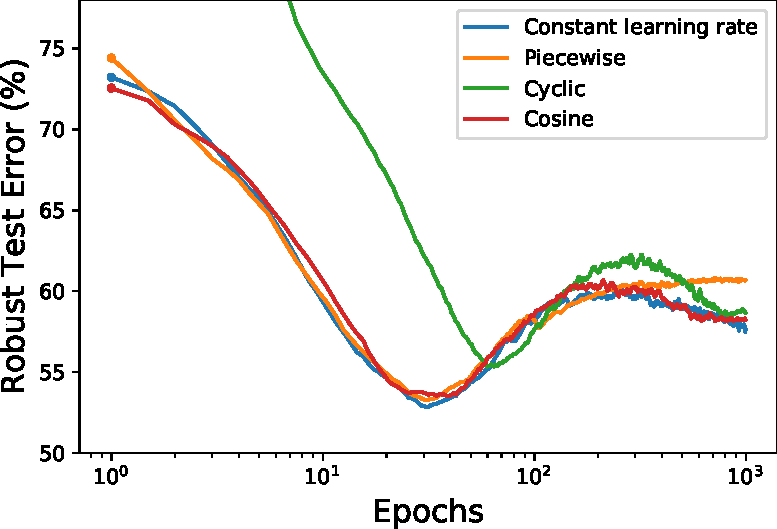
\includegraphics[width=0.45\textwidth]{figures/reconcile-lr-scheduler.pdf}
%   \caption{The effect of the learning rate scheduler on the epoch-wise double descent curve in adversarial training. Modulating the model capacity can produce training curves with diverse behaviors. Different model architectures may produce slightly different double descent curves. The training curve is smoothed by moving average with a window of $5$.
%   }
% \label{fig:reconcile-lr-scheduler}
% \end{figure*}

% \smallsection{Regularization}
% \subsection{\chengyu{Bias-variance analysis of adversarial training}}


% version https://git-lfs.github.com/spec/v1
oid sha256:21e6d7ec228b1a541a47be7af0bd934ed9a0f34a1749875e562206e0445a39f9
size 9061

% 
\subsection{Model-wise double descent in adversarial training}
\label{sect:model-wise-double-descent}
\todo{Move model-wise of number of attacks in the above to here}

We have shown that the epoch-wise double descent, which is connected to the robust overfitting, is strongly dependent on the data. Here we show that the model-wise double descent, a parallel type of double descent, is dependent on the data in a similar manner. This is thus aligned with our theoretical analysis of the dependence of the implicit label noise.

In Figure~\ref{fig:dependence-model-wise-perturbation-quality}, we control the model capacity by modulating the widening factor of a Wide ResNet, and produce the model-wise double descent by picking the robust test accuracy at the last checkpoint. One can find the model-wise double descent becomes more significant as the perturbation radius increases. Interestingly, when the perturbation radius is smaller than $4/255$, the robust overfitting gap (the gap between the last error and the best error obtained throughout the training) will eventually close as the model capacity is sufficiently large. This is consistent with the phenomenon observed in the epoch-wise double descent that the last error will be as low as the best error when the perturbation radius is small. 
% since large model will be effectively over-parameterized at the very beginning of the training.
One can expect the same phenomenon happens for a typical perturbation radius such as $8/255$ with extremely large models. This suggests the robust overfitting might not be inevitable as claimed in previous works~\citep{Rice2020OverfittingIA}, but just because the current model in practice is still under-parameterized for adversarially robust learning. 

Similarly, the model-wise double descent also becomes more significant as the data quality degrades. When the data quality is high, the robust overfitting gap is also gradually closed as the model capacity increases. % Similar observation has been made in recent works~\citep{Dong2021DataPF}.
% These suggest that the robust overfitting is only transient in terms of both the training time and the model capacity.

\begin{figure*}[!ht]
  \centering
  \includegraphics[width=0.9\textwidth]{figures/dependence-model-wise-perturbation-quality.pdf}
  \caption{(Left) Dependence of model-wise double descent on the perturbation radius. 
  $\varepsilon = 0/255$ indicates the standard training where no double descent occurs. 
  (Right) Dependence of model-wise double descent on the data quality. The solid and dashed curves indicate the error at the best and last checkpoints, respectively.
  }
\label{fig:dependence-model-wise-perturbation-quality}
\end{figure*}






% version https://git-lfs.github.com/spec/v1
oid sha256:d7370b8d68c42cd3b7e2217d91e192b30ebf952537885002ad4bb239e60e833d
size 2901

% % \subsection{Static adversarial perturbation}
% \label{sect:exp-static}

\smallsection{Adversarial augmentation}
We first obtain a robust model by conduct PGD training with pre-activation ResNet-18 on CIFAR-10. We use early stopping to obtain the most robust model on a validation set. The specific settings are aligned with Section~\ref{sect: exp-practical}.

Using this model, we then generate adversarial examples with PGD attack on the $5000$ examples randomly sampled from CIFAR-10 training set. The number of attack iterations is fixed as $10$ and the step size is fixed as $2/255$. The adversarial examples along with their original labels are then grouped into a training set for adversarial augmentation experiments.




% version https://git-lfs.github.com/spec/v1
oid sha256:122051f2431a5b436b094ebddc345f4fd484efcc0a36baa1a161ba0cc24b0baf
size 1294


version https://git-lfs.github.com/spec/v1
oid sha256:e72bab2b96cb5a401a7b14b64bb64b6c5206805e55e2320b228b193015f4d349
size 15194

\section{Study on a synthetic dataset with known true label distribution}
% \label{sect:synthetic}


% \note{2) change legends in figure 5 and table 1. Say $\rho=0$ is original dataset, $\rho=0.5$ is the traditional adversarial label, best model is the well-calirated model, last model is sth like the over-optimized model. 3) $\rho probably < 0.5$, like $\rho = 0.5 - \delta$.}

% \chengyu{Can move this section to appendix. or later part after the experiment results as some additional analysis of our method. }
% \chengyu{Or replace with similar experiments on cifar-10h}

    % Here, we empirically verify if the model probability can indeed approximate the true label distribution better than the traditional adversarial labels.
    
    \begin{wrapfigure}{r}{3cm} % [!ht]
    % \begin{figure} % {l}{3cm}% [!ht]
      \vspace{-3mm}
      \centering
      \includegraphics[width=0.2\textwidth]{figures/method-augment-image-example.pdf}
      \caption{Sample image by mixup augmentation.}
    \label{fig:method-augment-example}
    % \end{figure}
    \end{wrapfigure}
    
    \smallsection{Synthetic Dataset}
    Since the true label distribution is typically unknown for adversarial examples in real-world datasets, 
    we simulate the mechanism of implicit label noise in adversarial training from a feature learning perspective.
    Specifically, we adapt \emph{mixup}~\citep{Zhang2018mixupBE} for data augmentation on CIFAR-10. 
    For every example $x$ in the training set, we randomly select another example $x'$ in a different class and linearly interpolate them by a ratio $\rho$, namely $x:= \rho x + (1-\rho) x'$, which essentially perturbs $x$ with features from other classes. 
    Therefore, the true label distribution is arguably $y \sim \rho\cdot \mathbbm{1}(y) + (1-\rho)\cdot  \mathbbm{1}(y')$.
    Unlike mixup, we intentionally set the assigned label as $\hat{y} \sim \mathbbm{1}(y)$, thus deliberately create a mismatch between the true label distribution and the assigned label distribution.
    We refer this strategy as \emph{mixup augmentation} and only perform it once before the training. 
    % so we finalize the true distribution for every example.
    In this way, the true label distribution of every example in the synthetic dataset is fixed.
    % obtain a synthetic dataset with known true label distribution.
    
    % \begin{wrapfigure}{r}{5.5cm}% [!ht]
    %   \centering
    %   \includegraphics[width=1.0\linewidth]{figures/method-augment.pdf}
    %   \caption{Standard training on the synthetic dataset with $\rho=0.5$ and the original dataset (i.e., $\rho=0$). $(\cdot)$ in the legend indicates the distributions employed as the supervision. \jingbo{I don't think the legends here are clear enough. And it is not necessary to keep both best model and last model. We only need rho = 0, rho = 0.5 with assigned labels, rho = 0.5 with model probability. This will be enough to justify our points.}}%
    %   \label{fig:method-augment}
    % \end{wrapfigure}
    
    
%     \smallsection{Epoch-wise double descent can be observed on mixup augmentation}
%     In Figure~\ref{fig:method-augment}, we conduct standard training on the synthetic dataset with $\rho=0.5$ and the original dataset (i.e., $\rho = 0$) (See Appendix~\ref{sect: exp-mixup-augment} for experiment details). 
%     Compared with the training on the original dataset, the training on the synthetic dataset clearly exhibits an epoch-wise double descent, although no explicit label noise is injected into the dataset \jingbo{I'm a bit concerned here to say that no explicit label noise injected, because $\rho$ is 0.5. It will make me more comfortable if $\rho$ is strictly less than 0.5}, which further demonstrates the connection between the implicit label noise induced by distribution mismatch and the double descent phenomenon.


%     \smallsection{Model probability approximates the true label distribution}
%     Since we know the true label distribution in the synthetic dataset, we now quantitatively evaluate the approximation of model probability w.r.t. the true label distribution. 
%     We train a surrogate model on the same synthetic dataset to generate the probability. 
%     Since the true distribution is known, we can directly measure the distance between the model probability distribution and the true distribution. 
%     In addition to the total variation distance that measures the distribution mismatch, there are existing evaluation metrics in the literature such as \emph{calibration error}~\citep{Naeini2015ObtainingWC, Guo2017OnCO}, a measure specifically designed for classification algorithms, and \emph{proper scoring rules}~\citep{Gneiting2007StrictlyPS} such as negative log-likelihood (NLL) and Brier score~\citep{Brier1950VERIFICATIONOF} from a frequentist notion of uncertainty~\citep{Dawid1982TheWB, Degroot1983TheCA}. 
%     Instead of the label distribution, these metrics only requires the ground-truth hard label, which is accessible in an implicit label noise case since $\argmax_j p(\hat{y}=j|x) = \argmax_j p(y=j|x)$. 
%     Due to its simplicity and wide use in \emph{confidence calibration}~\citep{Guo2017OnCO}, we select the NLL loss on the validation set as a complementary metric to measure the quality of a approximate distribution. Smaller NLL loss means a better approximation to the true distribution. 
%     By Gibbs inequality, the NLL loss will be minimized when the model produces the true distribution.
%     Table~\ref{table: distance} shows the TV distance and the NLL loss to the true distribution of the model probability generated at the best checkpoint \jingbo{Do we have to emphasize the best vs. last? I think picking the best checkpoint is kind of common practice, assuming ``best'' is decided based on a dev set.} during training is significantly smaller than that of the assigned label.



% \begin{wraptable}{r}{7cm}
%   \caption{Average TV distance between the true label distribution and various approximate label distributions. The accuracy of the label distribution in terms of the argmax of the true label is also listed for reference.}
% \label{table: distance}
%   \small
%   \begin{tabular}{rlll}
%     \toprule
%     Distribution & Acc (\%) & TV & NLL (Val) \\
%     \midrule
%     Assigned label & 100  & 0.5 & - \\
%     Best Model & 80.24 & 0.4420 & 0.9504 \\
%     Last Model & 99.84 & 0.4996 & 2.7767 \\
%     \bottomrule
%   \end{tabular}
% \end{wraptable}

%     \smallsection{Employing model probability in training can mitigate double descent}
%     As suggested by Equation~(\ref{eq:loss-soft-label}), we simply substitute the one-hot label in the training objective by model probability with $T=1$ and $\rho=1$. 
%     Indeed, Figure~\ref{fig:method-augment} confirms that that employing the model at the best checkpoint as supervision can effectively mitigate the double descent. 
%     In contrast, the model at the last checkpoint cannot alleviate the double descent, which can also be reflected by the TV distance in Table~\ref{table: distance}, despite its high accuracy.
%     \jingbo{the following sentence may be not that important. Could be removed}
%     In Appendix~\ref{sect:better-approximate-mixup}, we show that the approximate label distribution modulated by the temperature and the interpolation ratio can further approach the true label distribution and mitigate the double descent more effectively.



% 
% \subsection{Synthetic dataset with Mixup augmentation}

\subsubsection{Better approximation with proper temperature and interpolation ratio}
\label{sect:better-approximate-mixup}

In Section~\ref{sect:synthetic} we show that on our synthetic dataset with known true distribution, namely mixup augmentation, the model probability can approach the true distribution. In light of our analyses in Section~\ref{sect:approximate-true-distribution}, here we show that with temperature $T$ and interpolation ratio $\lambda$, the model probability can approximate the true label distribution even better.

\smallsection{Temperature}
Here we focus on the effect of temperature on the model at the last checkpoint. We do not experiment on the model at the best checkpoint because we observe that $T=1$ is already near-optimal for best model in this experiment. As shown in Section~\ref{sect:synthetic}, the predictive probability of the model at the last checkpoint (or an overfitted model) cannot approximate the true label distribution well and thus it will produce double descent as significant as the assigned label. However, as shown in Table~\ref{table:augment-distance-temperature}, by properly set the temperature in the softmax function, the predicative probability can still approximate the true label distribution better than the assigned label. Consequently, it will also alleviate the double descent as shown in Figure~\ref{fig:method-augment-temperature}. Here the TV distance is smaller than the best model as we are considering all the examples thus the high accuracy plays a part.

% \chengyu{Best model worse than last model with temperature 10 in terms of TV because we consider all the examples here. Last model has much higher accuracy.}
% One can also find that the TV distance of the predictive distribution is almost as large as the assigned label, indicating a strong miscalibration. This shows quality uncertainty is more important than the accuracy when using predictive distribution as supervision. Interestingly, by tuning the temperature ($T=10$) for overfitted model, one can also better approach the true distribution. And as expected, this carefully selected temperature can help the model alleviate the double descent, which is consistent with our theoretical understanding.

% \begin{wrapfigure}{r}{5.5cm}% [!ht]
%   \centering
%   \includegraphics[width=1.0\linewidth]{figures/method-augment-temperature.pdf}
%   \caption{Test error yielded by standard training on the mixup augmented dataset.  $(\cdot)$ in the legend indicates the distributions employed as the supervision.}%
%   \label{fig:method-augment}
% \end{wrapfigure}

\begin{figure}[!ht]
\begin{floatrow}
\ffigbox{
  \includegraphics[width=1.0\linewidth]{figures/method-augment-temperature.pdf}
  \caption{Test error yielded by standard training on the mixup augmented dataset.  $(\cdot)$ in the legend indicates the distributions employed as the supervision.}%
  \label{fig:method-augment-temperature}
}
\hfill
\capbtabbox{%
  \small
  \begin{tabular}{rlll}
    \toprule
    % & \multicolumn{3}{c}{PGD} & \multicolumn{3}{c}{TRADES}\\
    % \cmidrule(lr){2-4} \cmidrule(lr){5-7}
    % & \specialcell{Robust\\(\%)} & \specialcell{Wall time\\(mins)} & \specialcell{Robust\\(\%)} & \specialcell{Wall time\\(mins)}\\
    Distribution & Acc (\%) & TV & NLL (Val) \\
    \midrule
    Assigned label & 100  & 0.5 & - \\
    \makecell{Last Model \\ ($T=1$)} & 99.84 & 0.4996 & 2.7767 \\
    \makecell{Last Model \\ ($T=10$)} & 99.84 & 0.4315 & 1.2297 \\
    % Last Model ($T$=2) & 99.88 & 0.4388\\
    % Last Model ($T$=10) & 99.84 & 0.4315 & \\
    \bottomrule
    % \tablefootnote{$^*$ indicates the best hyper-parameter searched.}
  \end{tabular}
}{%
  \vspace{8ex}
  \caption{Average TV distance between the true label distribution and various approximate label distributions. The accuracy of the label distribution in terms of the argmax of the true label is also listed for reference.
  % Experiment settings are specified in the text. Unless otherwise noted, we set the temperature to be $1$ in the softmax function, which recovers the original probability of the model.
  }
  \label{table:augment-distance-temperature}
}
\end{floatrow}
\end{figure}



% \begin{wrapfigure}{r}{5.5cm}% [!ht]
%   \centering
%   \includegraphics[width=1.0\linewidth]{figures/method-augment-temperature.pdf}
%   \caption{Test error yielded by standard training on the mixup augmented dataset.  $(\cdot)$ in the legend indicates the distributions employed as the supervision.}%
%   \label{fig:method-augment}
% \end{wrapfigure}






\smallsection{Interpolation ratio}
Now we validate if properly interpolating between model probability and assigned label can better approximate the true label distribution. As shown in Table~\ref{table:augment-distance-ratio}, a proper interpolation ratio can indeed produce a distribution that approaches the true label distribution closer than the model probability only\footnote{We use a surrogate model to calculate NLL loss for the assigned label, see Appendix~\ref{sect:confidence-calibration-assigned} for details.}. Consequently, it can mitigate the double descent more significantly and achieve better performance.




\begin{figure}[!ht]
\begin{floatrow}
\ffigbox{
  \includegraphics[width=1.0\linewidth]{figures/method-augment-ratio.pdf}
  \caption{Test error yielded by standard training on the mixup augmented dataset.  $(\cdot)$ in the legend indicates the distributions employed as the supervision.}%
  \label{fig:method-augment-ratio}
}
\hfill
\capbtabbox{%
  \small
  \begin{tabular}{rlll}
    \toprule
    % & \multicolumn{3}{c}{PGD} & \multicolumn{3}{c}{TRADES}\\
    % \cmidrule(lr){2-4} \cmidrule(lr){5-7}
    % & \specialcell{Robust\\(\%)} & \specialcell{Wall time\\(mins)} & \specialcell{Robust\\(\%)} & \specialcell{Wall time\\(mins)}\\
    Distribution & Acc (\%) & TV & NLL (Val) \\
    \midrule
    Assigned label & 100  & 0.5 & - \\
    \makecell{Best Model \\ ($\lambda=1.0$)} & 80.24 & 0.4420 & 0.9504 \\
    \makecell{Best Model \\ ($\lambda=0.8$)} & 91.09 & 0.3772 & 0.8930 \\
    \bottomrule
  \end{tabular}
}{%
  \vspace{8ex}
  \caption{Average TV distance between the true label distribution and various approximate label distributions. The accuracy of the label distribution in terms of the argmax of the true label is also listed for reference.
  }
  \label{table:augment-distance-ratio}
}
\end{floatrow}
\end{figure}



version https://git-lfs.github.com/spec/v1
oid sha256:6bf1fead23d23a30ed719c7e52974664c51739543a26c64b44656195508353f4
size 2407

version https://git-lfs.github.com/spec/v1
oid sha256:b2edfb452854a8e1f4e110f3a41818115a41f642221a6bac121bc6ac60f1ae2b
size 8760

\section{Experimental details}
\label{sect:exp-setting-all}

\subsection{Settings for main experiment results}
\label{sect: exp-practical}
\smallsection{Dataset}
We include experiment results on CIFAR-10, CIFAR-100, Tiny-ImageNet and SVHN.

\smallsection{Training setting}
We employ SGD as the optimizer. The batch size is fixed to 128. The momentum and weight decay are set to $0.9$ and $0.0005$ respectively. Other settings are listed as follows.
\begin{itemize}[leftmargin=*,nosep]
    \item CIFAR-10/CIFAR-100: we conduct the adversarial training for $160$ epochs, with the learning rate starting at $0.1$ and reduced by a factor of $10$ at the $80$ and $120$ epochs.
    \item Tiny-ImageNet: we conduct the adversarial training for $80$ epochs, with the learning rate starting at $0.1$ and reduced by a factor of $10$ at the $40$ and $60$ epochs.
    \item SVHN: we conduct the adversarial training for $80$ epochs, with the learning rate starting at $0.01$ (as suggested by \citep{chen2021robust}) and reduced by a factor of $10$ at the $40$ and $60$ epochs.
\end{itemize}

\smallsection{Adversary setting}
We conduct adversarial training with $\ell_\infty$ norm-bounded perturbations. We employ adversarial training methods including PGD-AT, TRADES and FGSM. We set the perturbation radius to be $8/255$. For PGD-AT and TRADES, the step size is $2/255$ and the number of attack iterations is $10$.
% We employ AutoAttack~\citep{Croce2020ReliableEO} For reliable robustness evaluation.


\smallsection{Robustness evaluation}
We consider the robustness against $\ell_\infty$ norm-bounded adversarial attack with perturbation radius $8/255$. We employ AutoAttack for reliable evaluation. We also include the evaluation results again PGD-1000, Square Attack and RayS.


\smallsection{Neural architectures}
We include experiments results on pre-activation ResNet-18, WRN-28-5, WRN-34-10 and VGG-19. 

\smallsection{Hardware}
We conduct experiments on 
% NVIDIA GeForce GTX 1080 Ti and 
NVIDIA Quadro RTX A6000.





% ----------------------------------------
\subsection{Settings for analyzing double descent in adversarial training}
\label{sect: exp-double-descent}

\smallsection{Dataset}
We conduct experiments on the CIFAR-10 dataset, without additional data.

\smallsection{Training setting}
We conduct the adversarial training for $1000$ epochs unless otherwise noted.
By default we use SGD as the optimizer with a fixed learning rate $0.1$. When we experiment on a subset (see below) we use the Adam optimizer to improve training stability, where the learning rate is fixed as $0.0001$.
% , since it requires minimal hyper-parameter tuning. 
The batch size will be fixed to $128$, and the momentum will be set as $0.9$ wherever necessary. No regularization such as weight decay is used. These settings are mostly aligned with the empirical analyse of double descent under standard training~\citep{Nakkiran2020DeepDD}.

\smallsection{Sample size}
To reduce the computation load demanded by an exponential number of training epochs, we reduce the size of the training set by randomly sampled a subset of size $5000$ from the original training set without replacement. 
% This will linearly shift the double descent curve but will not significant distort its shape as shown in Appendix~\ref{sect:double-descent-reconcile}. 
We adopt this setting for extensive experiments for analyzing the dependence of epoch-wise double descent on the perturbation radius and data quality (i.e. Figure~\ref{fig:dependence-perturbation-quality})..
% and the number of attack iterations.
% Note that in the experiment associated with data quality, we randomly sampled the training subset from those examples with quality lower than a threshold. 
% The sampled subset is restricted to class-balanced.

\smallsection{Adversary setting}
We conduct adversarial training with $\ell_\infty$ norm-bounded perturbations. We employ standard PGD training with the perturbation radius set to $8/255$ unless otherwise noted. The number of attack iterations is fixed as $10$, and the perturbation step size is fixed as $2/255$.
 
\smallsection{Robustness evaluation}
We consider the robustness against $\ell_\infty$ norm-bounded adversarial attack with perturbation radius $8/255$. We use PGD attack with $10$ attack iterations and step size set to $2/255$.



\smallsection{Neural architecture}
By default we experiment on Wide ResNet~\citep{Zagoruyko2016WideRN} with depth $28$ and widening factor $5$ (WRN-28-5) to speed up training. 

\smallsection{Hardware}
We conduct experiments on 
% NVIDIA GeForce GTX 1080 Ti and 
NVIDIA Quadro RTX A6000.

  
version https://git-lfs.github.com/spec/v1
oid sha256:122051f2431a5b436b094ebddc345f4fd484efcc0a36baa1a161ba0cc24b0baf
size 1294



% \subsection{Settings for adversarial augmentation}
% \label{sect: exp-ad-augment}




% \subsection{Settings for Mixup augmentation}
% \label{sect: exp-mixup-augment}

% For every example in the clean training set, we generate a perturbed training example by interpolating it with another example from a different class. All those perturbed examples along with their original labels are then grouped into a new training set, where we conduct standard training for $1000$ epochs. Other settings are same as those listed in Appendix~\ref{sect: exp-double-descent} except no adversary is employed.

\subsection{Settings for standard training on fixed augmented training sets}

\subsubsection{General settings for both adversarial augmentation and Gaussian augmentation}

\smallsection{Dataset}
We conduct experiments on the CIFAR-10 dataset, without additional data.

\smallsection{Training setting}
We conduct the standard training for $1000$ epochs.
We use Adam as the optimizer with a fixed learning rate $0.0001$ to improve training stability with a small training set (see below). The batch size will be fixed to $128$, and the momentum will be set as $0.9$ wherever necessary. No regularization such as weight decay is used.

\smallsection{Sample size}
To reduce the computation load demanded by an exponential number of training epochs, we reduce the size of the training set by randomly sampled a subset of size $5000$ from the original training set without replacement.

\smallsection{Neural architecture}
By default we experiment on Wide ResNet~\citep{Zagoruyko2016WideRN} with depth $28$ and widening factor $5$ (WRN-28-5).

\smallsection{Hardware}
We conduct experiments on 
% NVIDIA GeForce GTX 1080 Ti and 
NVIDIA Quadro RTX A6000.

\subsubsection{Construction of the training set}

% \subsection{Static adversarial perturbation}
% \label{sect:exp-static}

\smallsection{Adversarial augmentation}
We first obtain a robust model by conduct PGD training with pre-activation ResNet-18 on CIFAR-10. We use early stopping to obtain the most robust model on a validation set. The specific settings are aligned with Section~\ref{sect: exp-practical}.

Using this model, we then generate adversarial examples with PGD attack on the $5000$ examples randomly sampled from CIFAR-10 training set. The number of attack iterations is fixed as $10$ and the step size is fixed as $2/255$. The adversarial examples along with their original labels are then grouped into a training set for adversarial augmentation experiments.




version https://git-lfs.github.com/spec/v1
oid sha256:d7370b8d68c42cd3b7e2217d91e192b30ebf952537885002ad4bb239e60e833d
size 2901






\end{document}